\chapter[A Preliminary understanding of the global terrorism database]{Data understanding of GTD}
\chaptermark{Data understanding of GTD}

\section{Introduction to terrorism incident databases}
As part of a larger initiative to apply machine learning techniques to the study of terrorism a initial data understanding was taken as part of the data mining process.  CRISP-DM \citep{chapman2000crisp} was used which consists of six phases, these are:

\begin{enumerate}
\item Business understanding. This introductory step of the project is aimed at getting an understanding of the purpose of the project and resulting requisites from a business point of view and transforming these into data mining problem statement. 

In the context of this project the data  mining problem statement would be to investigate of the application of data mining techniques to the study of terrorism through the use of on-line terrorist incident  databases. Particularly this is the application of machine learning techniques to investigate underlying spatial, temporal, regional and attack vector type. Particularly to understand the methodologies that are most appropriate to the analysis of the data and to see what insights can be gained from these methodologies. 
\item Data understanding. This stage begins with a commencing assessment of the data involving a compiling of the data necessary to carry out the analysis after which a number of activities are carried out to gain a familiarity with the data, to establish if data quality issues exist within the data and to determine initial insights or to find compelling sub-populations within the data on which to construct a number of hypothesis on veiled or obfuscated information which may exist within the data. In the context of this investigation the data is provided by the GTD. The data quality problems associated  with the dataset are highlighted in section~\ref{sec:markermeasdif}.
\item Data preparation. This stage would traditionally deal with assembly of the full final dataset, however as the data was already was pre-assembled this stage was not required.  
\item Model building. During this stage a number of different modelling techniques are applied. To make the data applicable to the specific data mining techniques a number of data preparation tasks may be required so returning back to the data preparation step may be required.
\item Model evaluation. During this step the model construction and any insights gained from the model are evaluated.
\item Model Deployment. During this step the model is deployed in a production setting, however this stage is not applicable in the current setting. 
\end{enumerate}

\section{Data mining techniques used in the preliminary understanding of the GTD database data}
Preliminary analysis was used to gain an initial understanding of the GTD through the use of a number of geo-spatial, regio-specific and regio-temporal patterns this was done using a mix of descriptive visualization. Dimension reduction and preliminary modelling were also used to gain an understanding of the GTD but also to see which modelling techniques might applicable to its study. To avoid data dredging or 'post-hoc story telling' therefore a  broad range of different techniques were applied. These techniques included:
\begin{enumerate}
\item Data visualization. A number of data visualization techniques were used to gain an initial understanding of evolution of terrorism from a temporal, attack vector type and regional perspective. Unsupervised techniques, both hierarchical and k-means clustering, were utilized to gain a better understanding of spatio (particularly regio-specific attack types). These techniques were used in conjunction with both static and interactive visualization to enhance and ease analysis, particularly with the spatio clustering of terrorist incidents using leaflet \citep{leaflet2016}. To accomplish this, interactive spatial visualization in conjunction with clustering is used to show the concentration of terrorist incidents in urban areas. This section can be seen as a an extension of descriptive analytics using visualizations. Descriptive analytics can be seen as the most basic form of analytics as they allow alot of data to be condensed into smaller more effective and insightful packets of information. The purpose of the descriptive analytics is to provide more purposeful and useful information. The descriptive analytics are then visualized using an appropriate visualization technique or provided in
tabular format. Dimension reduction along with which can be seen as providing a higher level of data reduction and more insightful data. Both the creation of summary statistics and simple data visualization and dimension reduction  can be seen as a form of descriptive analytics. Both forms of descriptive analytics allow the analyst to uncover underlying patterns within the data.

\item Dimension reduction techniques. Dimension reduction techniques (in the context of this project this can be considered a unsupervised learning technique as opposed to a data pre-processing step) are used to gain a better understanding of the interaction between multiple data dimensions as with the data visualization techniques used as described above, are limited to a small number of dimensions (three to four dimensions). Dimension reduction techniques used in conjunction with interactive data visualization techniques  allow the researcher to gain a better insight into the data by allowing the ability to analyse multiple dimensions with many levels and drill deep into the data. This would not be possible with static data visualizations of the data as the visualizations would become crowded and difficult to understand. In this chapter correspondence (CA) and multiple correspondence analysis (MCA) \citep{factominer2008} are utilised to carry out dimension reduction on a number of categorical dimensions (CA and MCA can be seen as analogous to principal component analysis but for categorical data) and the results are then visualized using Plotly \citep{plotlymanual2016}. 
\item A number of preliminary modelling techniques are to used to gain a further understanding of the temporal spatial and attack vector types. A number of supervised methods particularly Poisson regression, Hidden Markov Models for the analysis of time series data of deaths due to terrorism. 
\end{enumerate}

\section{Data mining techniques used in the preliminary understanding of the GTD database data}
\label{sec:chap4dataprep}

A number of different visualization techniques were used to explore the temporal and spatio temporal relationships between deaths due to terrorism.  A number of different data visualizations techniques were used ranging from simple time series plots to stacked bar chart to various types of choropleths. Stacked bar plots were used to encode a third data dimension along with year and deaths due to terrorist incidents. The static plots were created with ggplot2 \citep{ggplotwickham2009}, Hadley Wickhams own implementation of the grammar of graphics \citep{wilkinson2006grammar}. Dplyr \citep{dplyr2016wickham}, reshape2 \citep{reshape2007wickham} and tidyr \citep{tidyr2916Wickham} is used to manipulate and transform the data before visualizing the data. Typical transformations used are aggregation of data and conforming data to the correct shape through wide to long or vice-versa transformations.

Googlevis (which is an r wrapper around google's visualization), Plotly \citep{plotlymanual2016} and leaflet \citep{leaflet2016} are used to create a number of interactive plots. Using leaflet and Googlevis to create interactive choropleths offers a number over traditional static methods as more information can be stored through the  use of interactive layers and captions which can display further information in call out boxes. 

\subsection{The evolution of terrorism over time (year and month) by
region and world wide}\label{sec:evteryearmonth}

Plotting the monthly totals of deaths due to terrorism by region and by
world wide figures,we see using these two plots , temporal and
regional-temporal relationships emerge. The relationships are shown in figures \ref{fig:tseriesmonth1} and \ref{fig:tseriesmonthregion1}
:

\begin{enumerate}
\item
  Since records have started to be recorded in 1970, deaths due
  terrorism is on the rise. From the time series world plot we see that
  during the 1980's there was a sharp rise in terrorism. This flattened
  out with end of the cold war and appears to be declining up to the end
  of 1990's, after September the 11th 2001 there is an increase in
  terrorism. This increases dramatically with the invasions of Iraq and
  Afghanistan, it increases upto 2007, before sharply rising after 2010.
\item
  When examining the time series plot by month by region, We see a more
  refined pattern. A spike in terrorism can be seen in the 1980's due
  to a sharp rise in terrorism in Central America and later in the
  decade in South America. This fell at the end of the 1980's and start
  of the 1990's. Terrorism fell across all regions before beginning to
  rise in the 2000's especially in sub-Saharan Africa, the middle east
  and North Africa and south Asia (particularly Afghanistan and
  Pakistan).
\end{enumerate}

The time series plot for the different regions is shown below. The
temporal, regional relationships described above are clearly visible.

\begin{figure}[t]
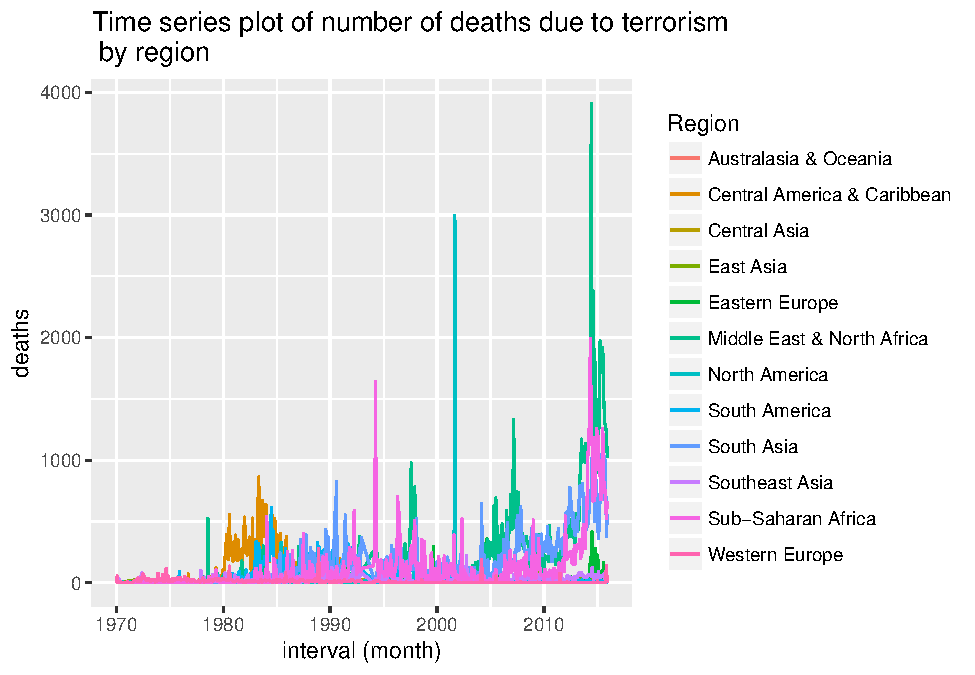
\includegraphics[width=10cm]{C:/Users/Peter/Desktop/Peters_experiment_markdown_files/figure-latex/unnamed-chunk-2-1.pdf}
\caption{Time series plot interval(month) of deaths by region}
\label{fig:tseriesmonthregion1}
\centering
\end{figure}

While the world wide time series plot quite clearly shows the rise in
terrorism worldwide since 1970. Plotting by region again the specific
temporal regional relationships are clearly visible, these are the sharp
rise in the 1980's to the start of the 1990's of deaths due to
terrorism. Again a regional shift of deaths due to terrorism has shifted
to the Middle East, this rose after the September 11th attacks and the
subsequent invasions of Afghanistan and Pakistan.

\begin{figure}[t]
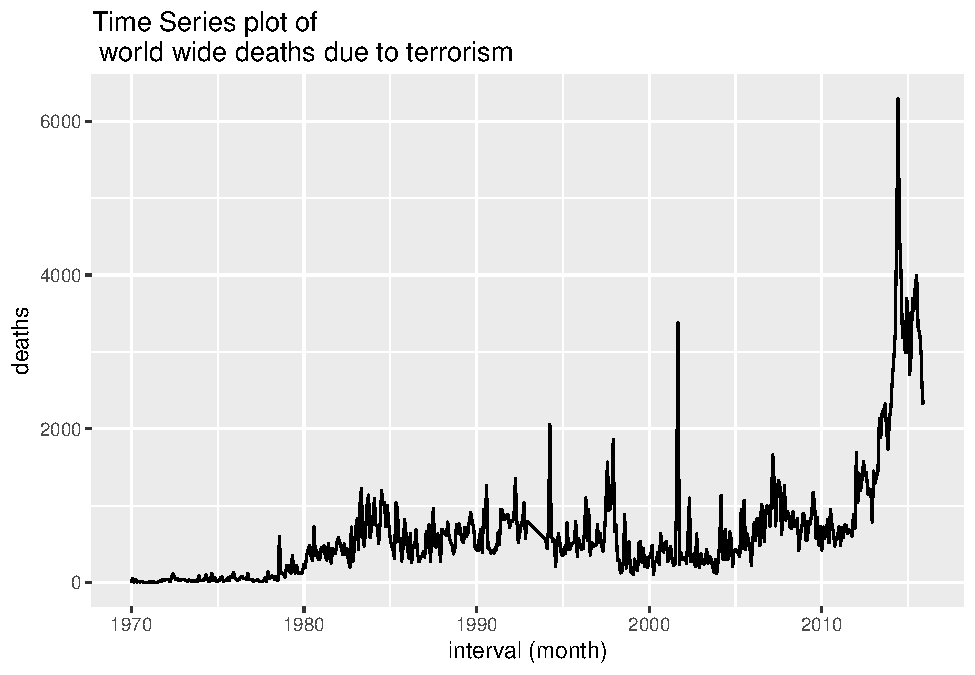
\includegraphics[width=10cm]{C:/Users/Peter/Desktop/Peters_experiment_markdown_files/figure-latex/unnamed-chunk-3-1.pdf}
\caption{Time series plot interval(month) of deaths}
\label{fig:tseriesmonth1}
\centering
\end{figure}

\subsection{The evolution of terrorism over time (year) by
region}

The rise in deaths to due to terrorism is more clearly observed when the global rise in deaths due terrorism by year since 1970, using a year interval instead of month interval (which was used in the previous section~\ref{sec:evteryearmonth}). The pattern is even more clearer the time series of deaths by years and deaths by year and region is plotted. Figure~\ref{fig:tseriesyear1} shows the number of deaths globally (not broken out by region). A rise in the late 1970's and 1980's followed by a period of relative stabilization  which persisted till the early 2000's followed by a large increase thereafter.

\begin{figure}[t]
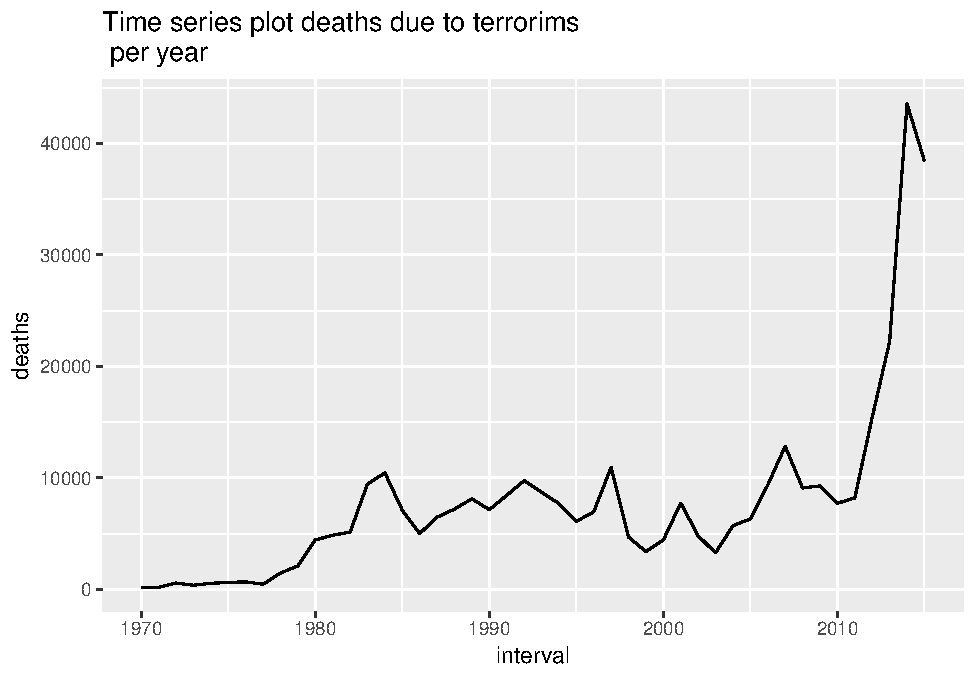
\includegraphics[width=10cm]{Peters_experiment_markdown_files/figure-latex/unnamed-chunk-4-1.pdf}
\caption{Time series plot interval(year) of deaths}
\label{fig:tseriesyear1}
\centering
\end{figure}

When viewing these deaths by  year and region. A clear pattern emerges the rise in number of deaths due to terrorism in Central America in the 1980's which fell
sharply towards the end of the cold war. A rise in terrorism is also clearly  visible post the September the 11th attacks in North Africa and the Middle East and in South Asia, Figure~\ref{fig:tseriesyear2}.

\begin{figure}[t]
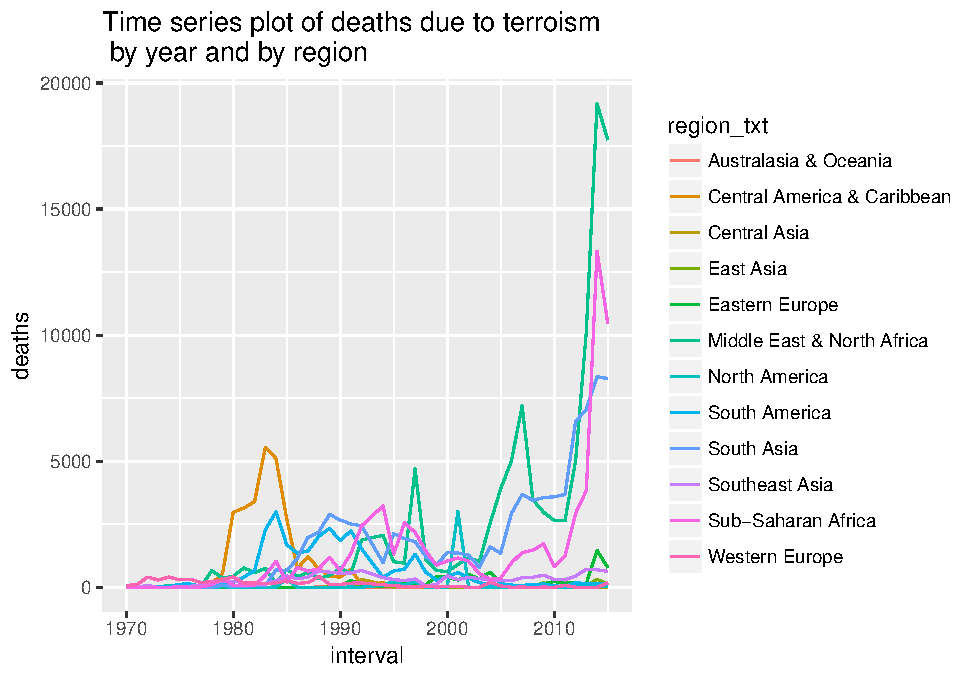
\includegraphics[width=10cm]{Peters_experiment_markdown_files/figure-latex/unnamed-chunk-5-1.pdf}
\caption{Time series plot interval(year) of deaths}
\label{fig:tseriesyear2}
\centering
\end{figure}

The regio-temporal shifts are even more evident when visualizing the  data as a stacked bar chart, Figure~{fig:stackbaryear1}. The stacked bar chart lets us assess the contributing fraction of total deaths for a particular time interval.When viewed as a stacked bar plot (with the region represented as portion of the bar). It is clear to see the fall off in terrorism in South America and Central America (the 1990's), corresponding with a rise in deaths due to terrorism in the Middle East and South
Asia. For the last decade the number of deaths that are due to terrorism
has been dominated by South Asia, the Middle East and Sub Saharan
Africa. Note the gap at 1993 due to the loss of data from the GTD when transferring data from the Pinkerton agency to the GTD.

\begin{figure}[t]
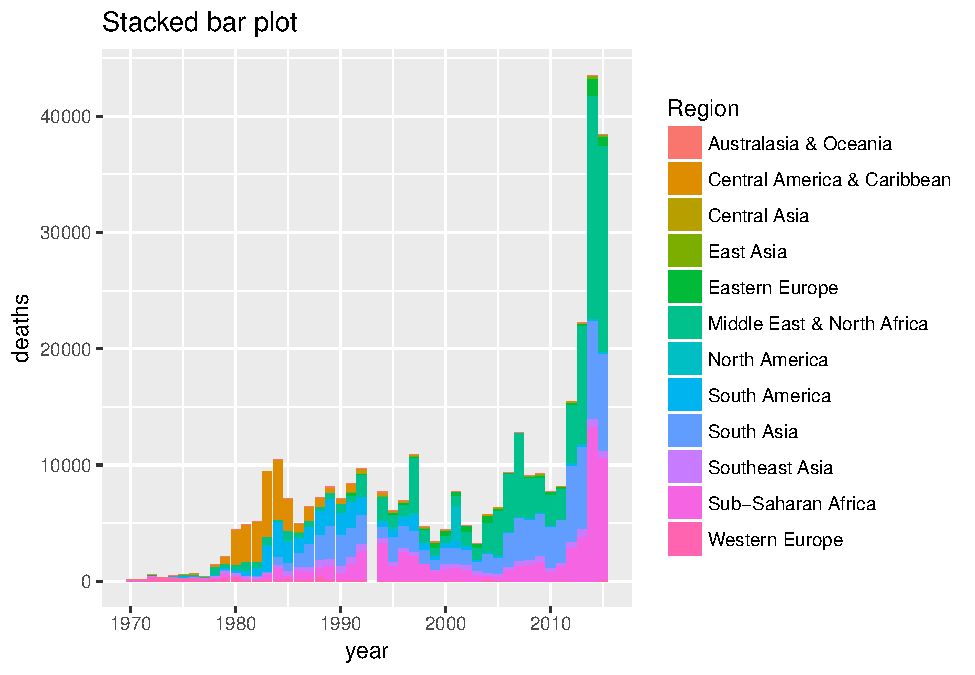
\includegraphics[width=10cm]{Peters_experiment_markdown_files/figure-latex/unnamed-chunk-6-1.pdf}
\caption{Stacked bar plot interval(year) of deaths}
\label{fig:stackbaryear1}
\centering
\end{figure}

\subsection{Visualizing deaths by attack vector and weapon type
type}\label{viewing-deaths-by-attack-vector-type}

Examining the plot of deaths due to attack vector (armed assault,
Hijacking, hostage taking etc) is shown below. Again a temporal
relationship exists,since the 2000's emergence of bombings and explosives
as the prominent attack vector. Also the emergence of hostage taking
(barricade incidents and Kidnapping).

\begin{figure}[t]
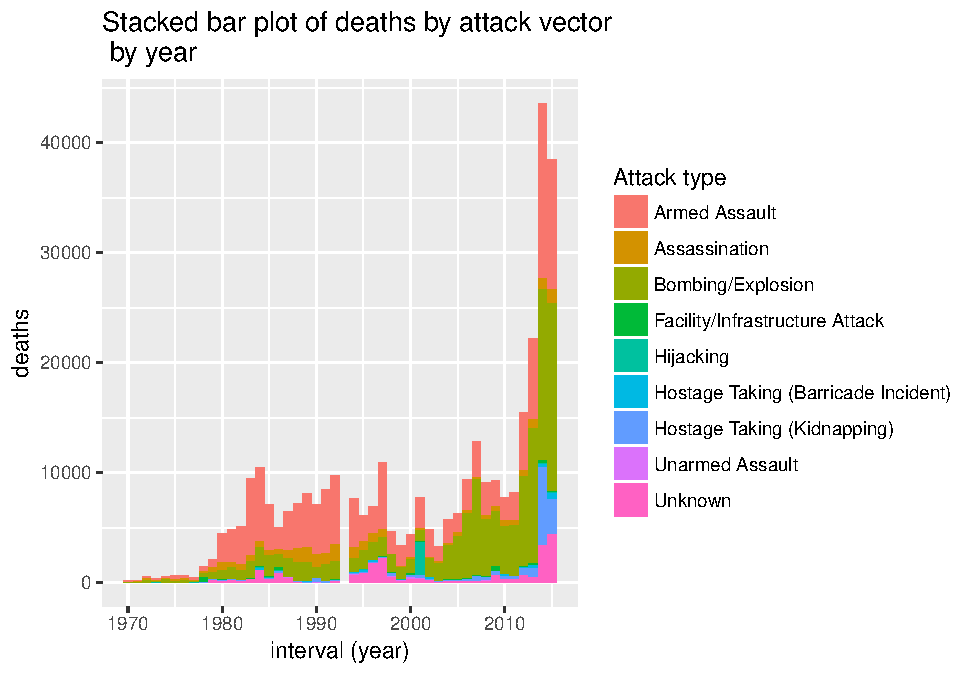
\includegraphics[width=10cm]{Peters_experiment_markdown_files/figure-latex/unnamed-chunk-7-1.pdf}
\caption{Stacked bar plot interval(year) of deaths by regions}
\label{fig:stackbaryearattackvector1}
\centering
\end{figure}

A similar trend is observed when we just look at the Middle east, with the dominating attack vector type being bombings and explosions the attack vector.

\begin{figure}[t]
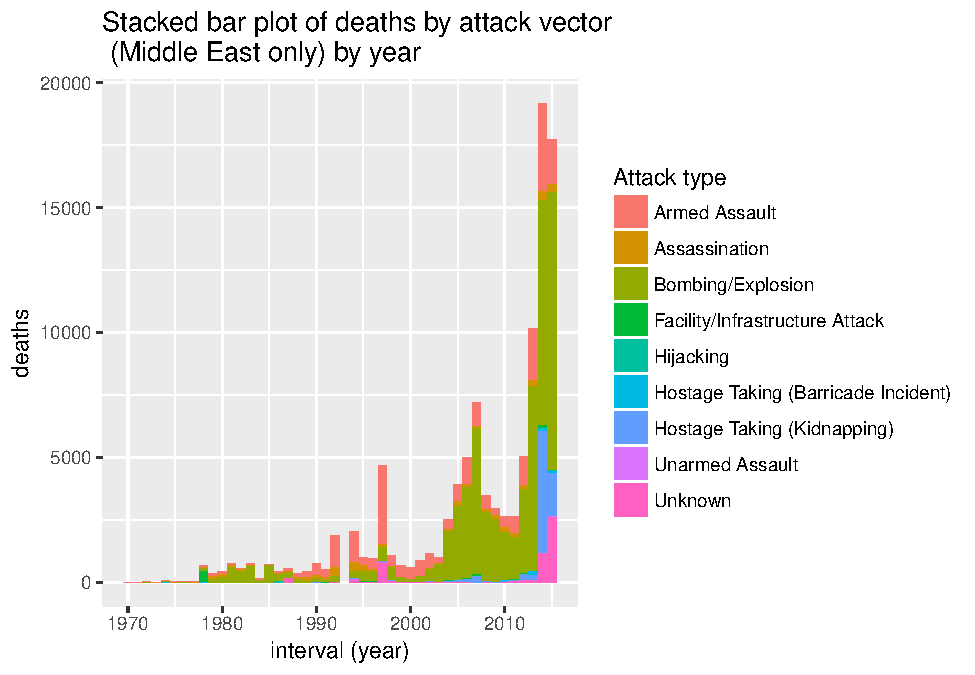
\includegraphics[width=10cm]{Peters_experiment_markdown_files/figure-latex/unnamed-chunk-8-1.pdf}
\caption{Stacked bar plot interval(year) of deaths by weapon type in the Middle East and North Africa}
\label{fig:stackbaryearattackvectormideast}
\centering
\end{figure}

When visualizing by attack type by interval year we can see a clear pattern emerge. Up until the early 2000's the dominant weapon type used was firearms, hover after this period explosives began to be the preeminent attack type. 

\begin{figure}[t]
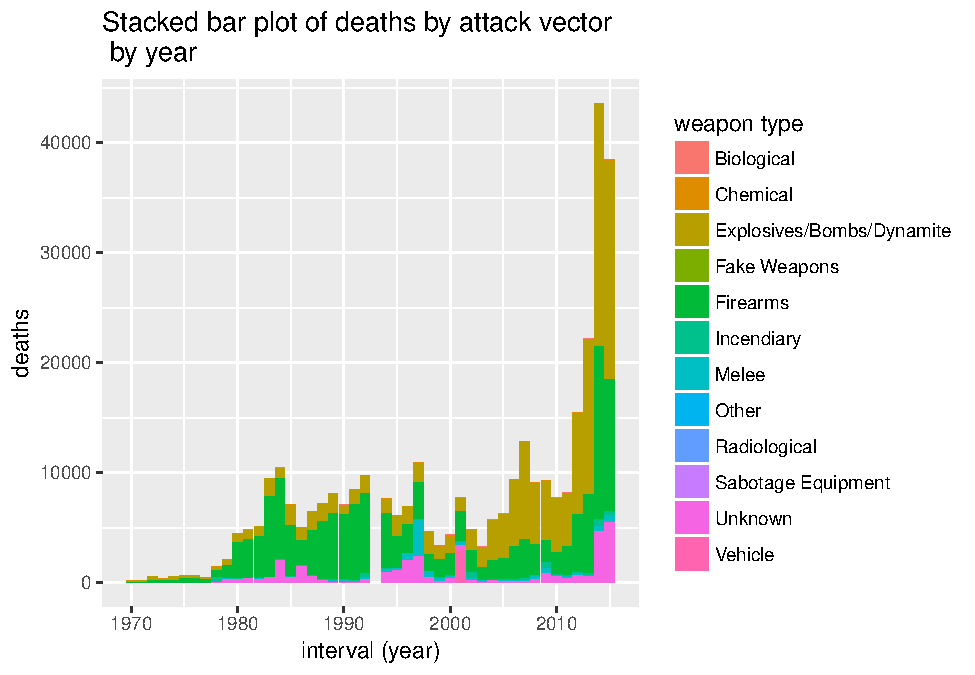
\includegraphics[width=10cm]{Peters_experiment_markdown_files/figure-latex/unnamed-chunk-9-1.pdf}
\caption{Stacked bar plot interval(year) of deaths by attack type}
\label{fig:stackbaryearweaptype}
\centering
\end{figure}

\subsection{Visualizing deaths by country and decade 
type}\label{viewing-deaths-by-attack-vector-type}

Previously the relationship by year and region had shown a regio-temporal shift in death due to terrorism (see section~\ref{sec:evteryearmonth}). By creating a stacked choropleth. The number of Deaths by Decade (1970's,1980's,1990's,2000's,2010's) are visualized as a stacked choropleth, see figure~\ref{fig:choroplethdecade}. Again the regio-temporal shift in deaths can be seen. In the 1970's terrorism was not particularly associated with no one particular region. Britain, Spain, Italy, USA, Nicaragua, Colombia, Philippines and Argentina show the largest number of Deaths due to terrorism.In the 1980's a clear regio-specific pattern can be seem concentrated in Central and South America, particularly in Nicaragua, Guatemala and Colombia.
In the 1990's no clear regio-specific pattern is seen with deaths due to terrorism being widely dispersed through out the World, though large scale deaths due to terrorism persisting in Colombia and Ecuador, Algeria emerging as a prominent country along with Southern Africa particularly (Angola, Mozambique and  South Africa) and  Turkey and Russia. 
The 2000's sees a large increase in deaths in the US, Iraq, Russia, Afghanistan and Pakistan, but shows large decreases in India and Algeria. As well as an almost total disappearance of terror from Southern Africa and Columbia and Ecuador.

\begin{figure}[t]
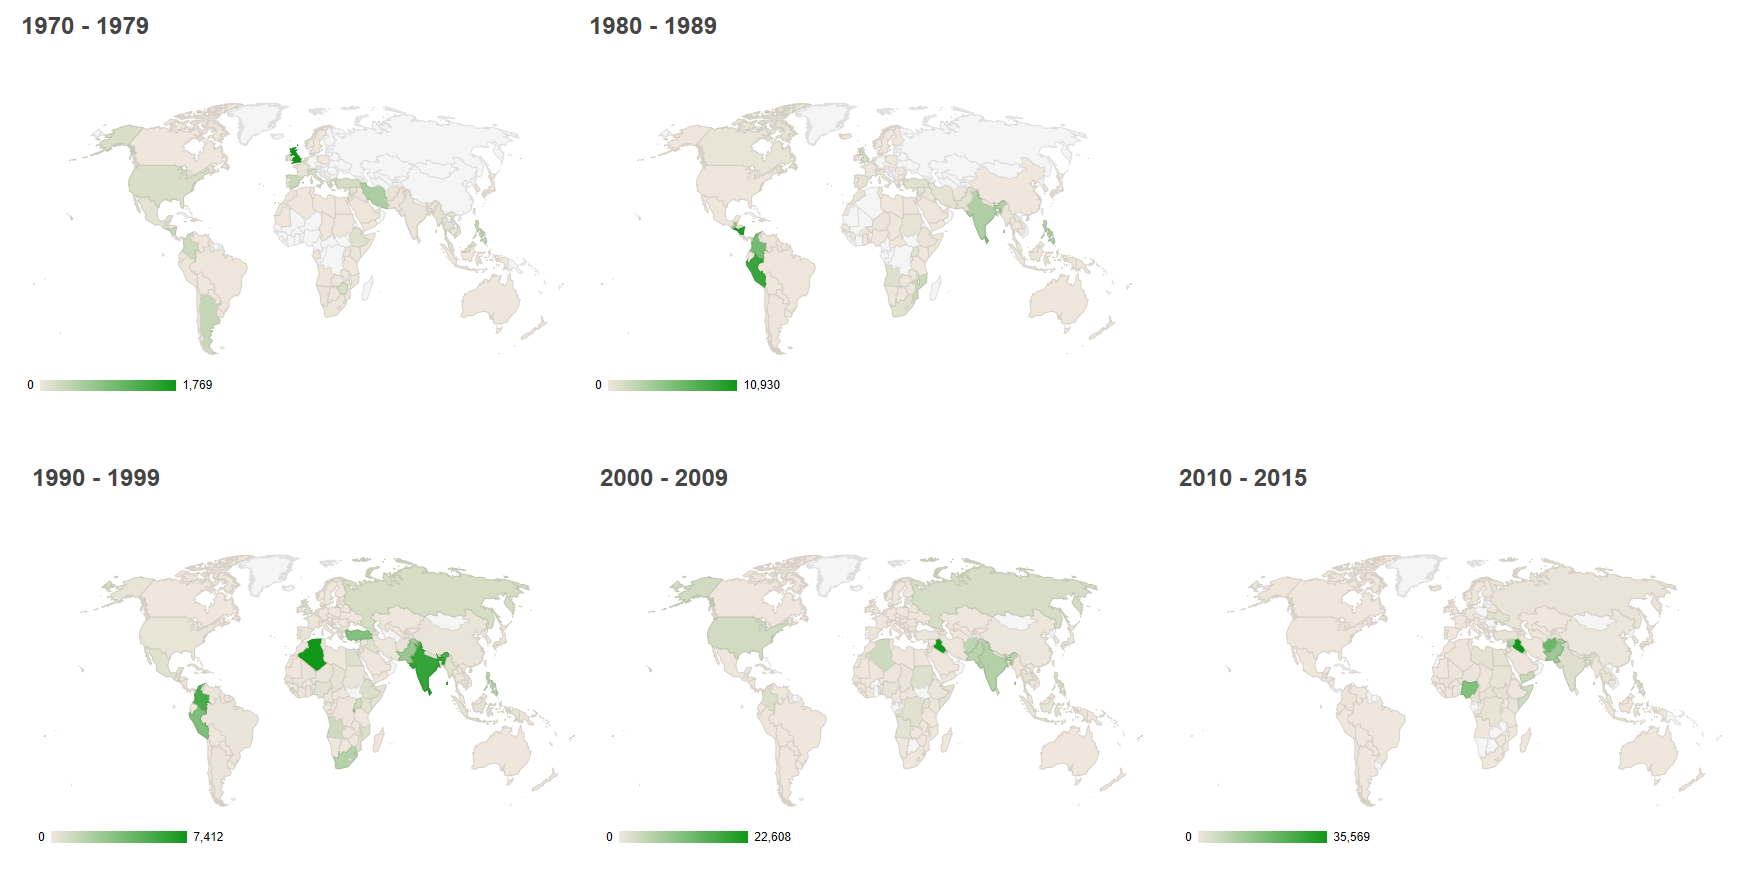
\includegraphics[width=15cm,height=15cm]{Peters_experiment_markdown_files/figure-latex/Capture_Choropleth_By_Decade_Deaths.png}
\caption{A stacked choropleth showing deaths by decade due to terrorism.}
\label{fig:choroplethdecade}
\centering
\end{figure}

\subsection{Visualizing deaths by rural urban 
categorization using K-means and Kernel Density estimation and interactive maps to create heatmaps} \label{viewing-deaths-by-K-means_Iraq_Syria}
In the previous sections(\ref:{section:viewing-deaths-by-attack-vector-type} and \ref{sec:evteryearmonth}) it could be quite clearly seen that South Asia (particularly Afghanistan) and the Middle East (particularly Iraq and Syria). Iraq was chosen for further analysis as it has been (since the invasion of Iraq in 2003), the country which consistenly ranks first in terms of deaths due to terrorism. Syria, since the Arab spring and the ensuing rebellion against the Assad regime of 2012 (\citep{dabashi2012arab}) led to the rise of ISIS and the establishment of a caliphate across certain parts of Iraq and Syria. These countries due to the pre-eminence of terrorist activities in these countries, led to their selection for further analysis.

Analysis at a finer grain can be carried out by using a combination of K-Means clustering, Kernel density estimation and interactive visualization for Iraq and Syria to examine if a rural urban divide (are attacks focussed in one specific area and are they associated with rural or urban areas) exists. To do this Iraq and Syria were chosen and the data was limited to Syria and Iraq for 2015. Density estimation creates a fundamental estimate of the probability density function, kernel density estimation creates a smooth kernel function for all data points then aggregating these to get a density estimate. The fundamental kernel estimator is given by the equation \ref{eq:eq1kernelest}.

\begin{equation} \hat{f}_{kde} = 1/n \sum^n_{i=1} K((x-x_i)/h) \label{eq:eq1kernelest}  \end{equation}

\begin{equation} MISE(\hat{f})=E[\int(\hat{f}(x)-f(x))^2 \ dx]
\label{eq:eq1l2risk}  \end{equation}
Where:
\begin{itemize}
\item[]  Where $K$ is the kernel which is a symmetric, positive function which sums to one. Typical kernel function are uniform triangle, normal and cosine.
\item[]  Where $h$ is the bandwidth which is a smoothing parameter, large bandwidths create extremely smooth estimates while the  converse is true for small bandwidths which produce noisy estimates, as the smoothing tends to impact the estimates much more so than the choice of kernel, it is imperative to determine the optimum bandwidth. The bandwidth is usually chosen by reducing to a minimum the mean integrated square error, given by the equation \ref{eq:eq1l2risk}.
\end{itemize}

The bkde2d function of the Kernsmooth package is used to calculate the 2d kernel density estimate based upon the WGS84 coordiantes of the terrorist incidents, linear binning is then used to create a series of bin counts and a 'Fast Fourier Transform (FFT)' is then utilized to carry out a a series of discrete convolutions. A bivariate Gaussian kernel concentrated at the specific location and the heights of the kernel scaled by the bandwidths are then calculated and aggregated at every datapoint. This allows the creation of heatmaps by overlaying the density estimates on map created using leaflet. The resulting map which overlays the points on to of the density estimates shows that n Iraq the incidents are largely concentrated around Baghdad while in Syria the incidents appear to be concentrated around the city of Allepo, figure~\ref{fig:iraqsyriakde}. To gain a greater understanding of the of spatial distribution of incidents K-Means clustering was also used.


K-means clustering aims to divide a number of into k number of clusters and is one of the easiest to understand and popular implementations of clustering. The number of clusters is decided apriori, metrics can be used to guide to the choice of K which minimize inter observation distance within clusters and maximize the distance between clusters. Such metrics include Davis Bouldin index \citep{davies1979cluster}. Alternately useful values for K can be chosen on whether the clusters make sense to the analyst based on expert knowledge. The algorithm can be summarized using the subsequent  stages:
\begin{enumerate}
\item K points are arranged into the space characterized by the observations that are being clustered. These points are defined as the first cluster centroids.
\item For all observations they are assigned to the cluster with the nearest centroid.
\item Upon all observations being designated to a particular cluster, the location of the cluster centroids are determined.
\item Stages 2 and 3 are repeated until the centroids no longer change position. This produces a separation of the objects into groups from which the metric to be minimized can be calculated.
\end{enumerate}
Succinctly put, the K-Means algorithm goal is to minimize an objective function a squared error function given by the formula \ref{eq:eq1kmeans}, 

\begin{equation} J=\sum_{j=1}^{k}\sum_{i=1}^{n}\left \| x_{i}^{j} - c_{j} \right \|^{2} \label{eq:eq1kmeans}  \end{equation}

Where the formula \ref{eq:eq1kmeans} represents the distance metric between a specific observation and the cluster centre. 

\begin{equation} \| x_{i}^{j} - c_{j} \|^{2}  \label{eq:eq2kmeans}  \end{equation}

In the case of clustering  a set of longitude/latitude locations the a great circle distance matrix is calculated for all couples of longitude/latitude using the haversine method (equation \ref{eq:haversine1}) where \textit{h} is haversine (equation \ref{eq:haversine2}). Solving equation \ref{eq:haversine1} by applying the inverse of the haversine equation \ref{eq:haversine3}) is derived.  

\begin{equation} d = r hav^{-1}(h) - 2r\arcsin(\sqrt{h})  \label{eq:haversine1}  \end{equation}

\begin{equation} hav(\frac{d}{r}) =hav(\varphi_{2}-\varphi_{1})+cos(\varphi_{2})hav(\lambda_{2}-\lambda_{2})  \label{eq:haversine2}  \end{equation}

\begin{equation} d=2r \arcsin(\sqrt(sin^{2}(\frac{\varphi_2-\varphi_1}{2})+cos(\varphi_2)sin^{2}(\frac{\lambda_2-\lambda_1}{2}))  \label{eq:haversine3}  \end{equation}

Where:
\begin{itemize}
\item[]  $hav$ is the haversine function given by $hav(\theta)=sin^2(\frac{\theta}{2})=\frac{1-cos(\theta)}{2}$
\item[] r gives the radius of the sphere.
\item[] $\varphi_1, \varphi_2$: represent latitude of observation 1 and latitude of observation 2, in radians, note in fields the rdist.earth function used to calculate the distance matrix in the fields package \ref{fields2015Nychka}, carries out a conversion from WGS84 \citep{misra1996integrated} to radians.
\item[]  $\lambda_1,\lambda_2$: represent the longitude of observation 1 and observation of point 2, in radians, note again in fields the rdist.earth function carries out a conversion from WGS84 \citep{misra1996integrated} to radians.
\end{itemize}

From figure~\ref{fig:iraqsyriakde}, it can be seen from the overlaying of the binned kernel density of the probability of incidents (estimated from latitude and longitude of the incidents) that the incidents in Iraq are concentrated in Western Iraq specifically around Baghdad and the Sunni triangle \citep{rand2015iraq} of Tikrit, Ar Raamdi and Baghdad which are the most densely populated areas of Iraq and inhabited mostly by Sunni Muslims, which became the centre for armed resistance Sunni opposition to the 2003 of Iraq \citep{hashim2005insurgency}, figure~\ref{fig:kmeansSyriaIraqSunniTriangle}. In Syria the incidents are concentrated around Aleppo, Homs, Latakia and Damascus. The clusters relating to these highly urbanized areas are categorized as being tightly grouped together as opposed to the clusters covering the Iraqi Western Desert and the Syrian Eastern Desert which are sparsely populated, figure~\ref{fig:kmeansSyriaIraq}.

\begin{figure}[t]
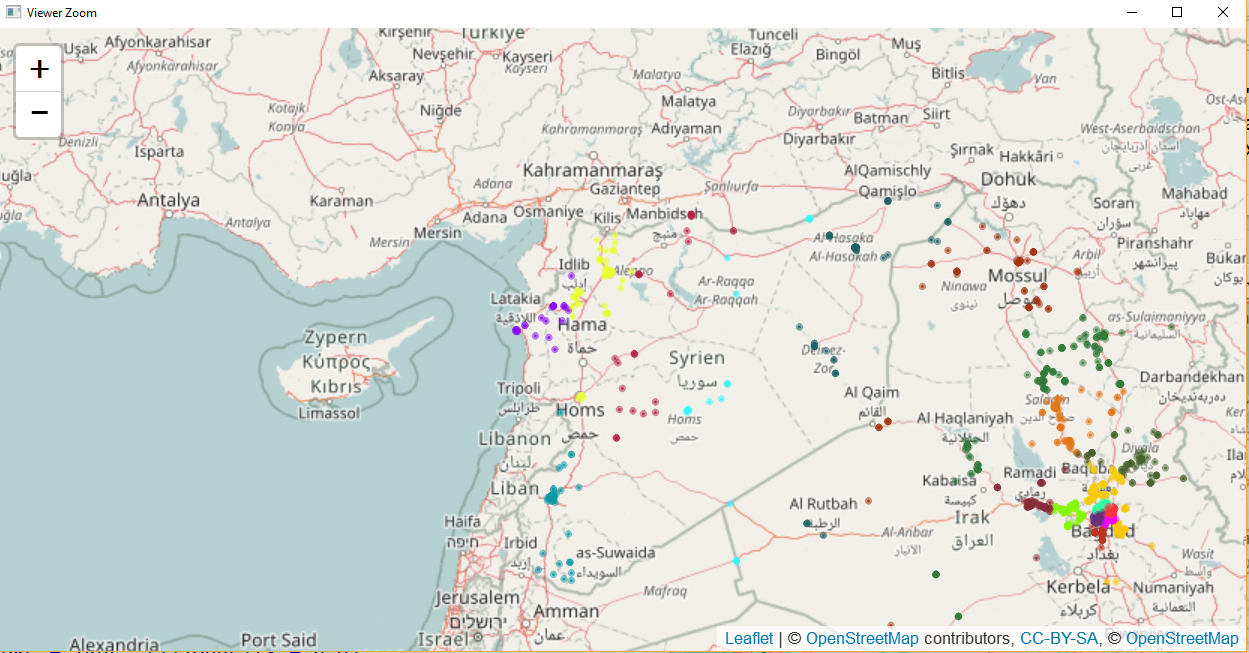
\includegraphics[width=15cm,height=15cm]{Peters_experiment_markdown_files/figure-latex/Capture_Kmeans_Leaflet_2015_Deaths_Iraq_Syria_K20.png}
\caption{Clustering of Terrorist incidents in Syria and Iraq}
\label{fig:kmeansSyriaIraq}
\centering
\end{figure} 

\begin{figure}[t]
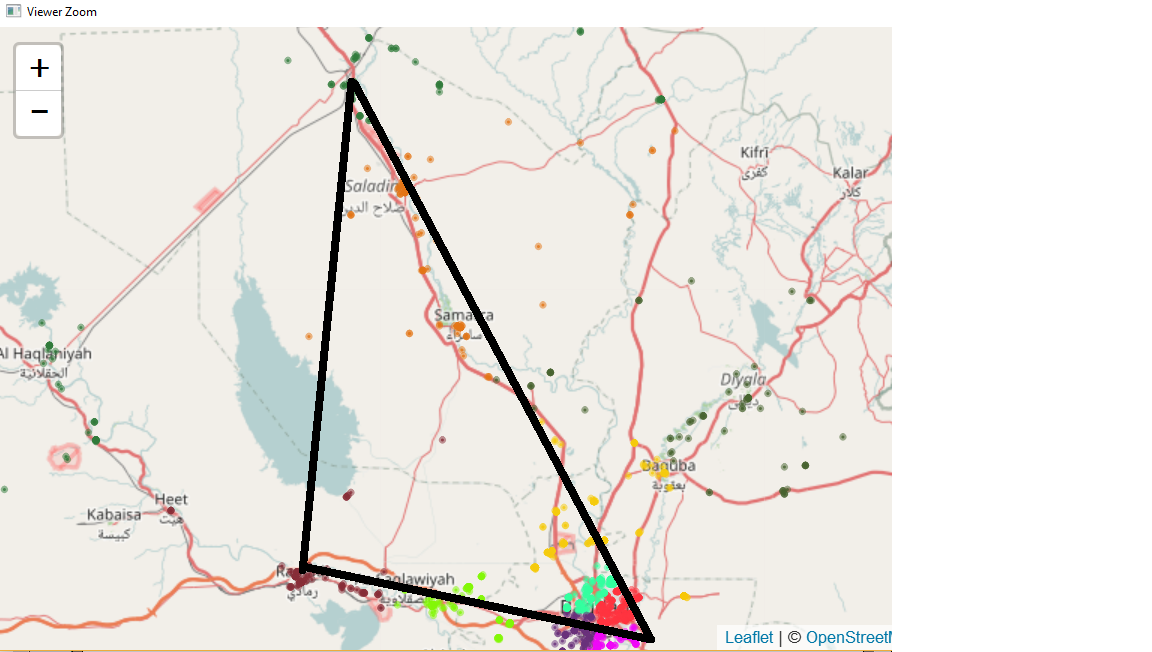
\includegraphics[width=15cm]{Peters_experiment_markdown_files/figure-latex/Capture_Kmeans_Leaflet_2015_Deaths_Iraq_Syria_K20_Sunni_Triangle_2.png}
\caption{Clustering of Terrorist incidents in Syria and Iraq, centred on the Sunni triangle}
\label{fig:kmeansSyriaIraqSunniTriangle}
\centering
\end{figure}

\begin{figure}[t]
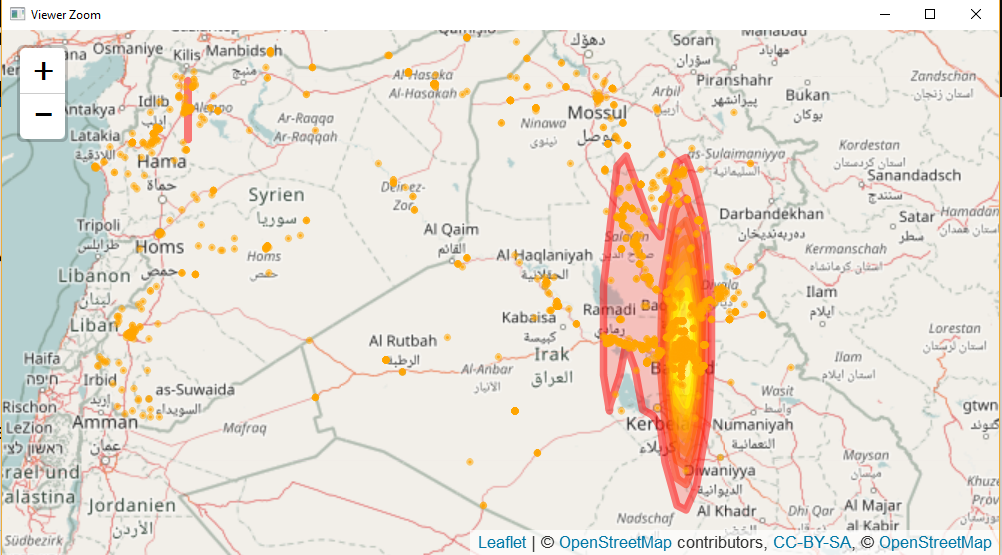
\includegraphics[width=15cm]{Peters_experiment_markdown_files/figure-latex/Capture_KDE_Leaflet_2015_Deaths_Iraq_Syria.png}
\caption{Heatmap of terrorist incidents in Syria and Iraq}
\label{fig:iraqsyriakde}
\centering
\end{figure}
 
\section{The use of dimension reduction techniques and clustering in understanding the GTD}\label{viewing-deaths-by-attack-vector-type} 

While the previous section largely utilised simple descriptive data visualizations to uncover underlying patterns in the data, these visualizations are limited in the number of data dimensions they can encode. To overcome this dimension reduction techniques (particularly Correspondence Analysis (CA) and Multiple Correspondence Analysis (MCA)) are used to reduce the data down from n dimensions to a more lower level while still maintaining the underlying structure in the data. These techniques can also be considered descriptive analytical techniques but are not limited to a low number of dimensions. CA (and MCA) is used in conjunction with D3 \citep{bostock2012d3} based interactive visualizations, using plotly \citep{plotlymanual2016} accessed through the R plotly package to create the bi-plots of the output of the analysis. This is done to aid navigation of the data and to ease understanding of many level categorical variables, which may appear crowded otherwise and difficult to understand. The reason correspondence is so appropriate to the study is the type of  data, which is largely categorical in nature.

CA is a multivariate statistical technique which is notionally similar to the more well known dimension reduction technique. It is used as a statistical visualization for envisaging the the associations (note the phrase correspondence comes from the french 'Analyses des Correspondances' where correspondence signifies a "system of associations" which exist between the different items which make up the two sets of data) or relationships between the different levels of a two way cross-tab table \citep{husson2010exploratory}. Two-way contingency tables are utilized in statistics to show how the perceived associations of two attributes (represented as rows and columns) displayed as cell frequencies of a matrix. An archetypical task within inferential statistics is to  ascertain the level of association between levels of one variable and levels of the other variable. CA transforms the data held within rows and columns of a two way contingency table into a lower dimensional space so that the points of the rows and columns in the lower dimensional space are representative of their associations in the table. The mathematics of CA is explained previously in section \ref{sec:synglobalter}.  

\subsection{Correspondence analysis of weapon type by year}\label{viewing-deaths-by-weapon-vector-type-CA}

CA was used understand better both the relationship year and weapon type. The contingency table of number of deaths by years and weapon type is shown in table \ref{tab:weaponsyear}.

% latex table generated in R 3.3.2 by xtable 1.8-2 package
% Sat Jan 07 14:52:55 2017

\begin{sidewaystable}
\centering
\resizebox{\textwidth}{!}{%
\begin{tabular}{rrrrrrrrrrrrr}
  \hline
 & Biological & Chemical & Explosives/Bombs/Dynamite & Fake Weapons & Firearms & Incendiary & Melee & Other & Radiological & Sabotage Equipment & Unknown & Vehicle\\ 
  \hline
1970 & 0.00 & 0.00 & 97.00 & 0.00 & 45.00 & 14.00 & 0.00 & 0.00 & 0.00 & 0.00 & 14.00 & 1.00 \\ 
  1971 & 0.00 & 0.00 & 82.00 & 0.00 & 80.00 & 1.00 & 2.00 & 0.00 & 0.00 & 0.00 & 8.00 & 0.00 \\ 
  1972 & 0.00 & 0.00 & 260.00 & 0.00 & 289.00 & 3.00 & 5.00 & 0.00 & 0.00 & 0.00 & 9.00 & 0.00 \\ 
  1973 & 0.00 & 1.00 & 80.00 & 0.00 & 270.00 & 1.00 & 8.00 & 0.00 & 0.00 & 0.00 & 10.00 & 0.00 \\ 
  1974 & 0.00 & 0.00 & 270.00 & 0.00 & 246.00 & 0.00 & 4.00 & 0.00 & 0.00 & 0.00 & 22.00 & 0.00 \\ 
  1975 & 0.00 & 0.00 & 125.00 & 0.00 & 481.00 & 0.00 & 3.00 & 0.00 & 0.00 & 0.00 & 8.00 & 0.00 \\ 
  1976 & 0.00 & 0.00 & 231.00 & 0.00 & 395.00 & 9.00 & 12.00 & 0.00 & 0.00 & 0.00 & 25.00 & 0.00 \\ 
  1977 & 0.00 & 1.00 & 36.00 & 0.00 & 374.00 & 3.00 & 3.00 & 0.00 & 0.00 & 0.00 & 39.00 & 0.00 \\ 
  1978 & 0.00 & 0.00 & 292.00 & 0.00 & 618.00 & 436.00 & 11.00 & 0.00 & 0.00 & 0.00 & 102.00 & 0.00 \\ 
  1979 & 0.00 & 1.00 & 474.00 & 0.00 & 1150.00 & 39.00 & 14.00 & 0.00 & 0.00 & 0.00 & 422.00 & 0.00 \\ 
  1980 & 0.00 & 0.00 & 684.00 & 0.00 & 3293.00 & 96.00 & 17.00 & 0.00 & 0.00 & 0.00 & 338.00 & 0.00 \\ 
  1981 & 0.00 & 0.00 & 864.00 & 0.00 & 3495.00 & 21.00 & 4.00 & 0.00 & 0.00 & 3.00 & 464.00 & 0.00 \\ 
  1982 & 0.00 & 0.00 & 824.00 & 0.00 & 3832.00 & 15.00 & 82.00 & 0.00 & 0.00 & 0.00 & 382.00 & 0.00 \\ 
  1983 & 0.00 & 0.00 & 1504.00 & 0.00 & 7380.00 & 10.00 & 9.00 & 0.00 & 0.00 & 0.00 & 540.00 & 0.00 \\ 
  1984 & 0.00 & 1.00 & 852.00 & 0.00 & 7367.00 & 52.00 & 95.00 & 2.00 & 0.00 & 0.00 & 2077.00 & 3.00 \\ 
  1985 & 0.00 & 0.00 & 1845.00 & 0.00 & 4571.00 & 114.00 & 17.00 & 0.00 & 0.00 & 0.00 & 547.00 & 0.00 \\ 
  1986 & 0.00 & 0.00 & 1106.00 & 0.00 & 2240.00 & 40.00 & 34.00 & 0.00 & 0.00 & 25.00 & 1552.00 & 6.00 \\ 
  1987 & 0.00 & 19.00 & 1642.00 & 0.00 & 4107.00 & 37.00 & 64.00 & 0.00 & 0.00 & 0.00 & 609.00 & 0.00 \\ 
  1988 & 0.00 & 0.00 & 1530.00 & 0.00 & 5305.00 & 22.00 & 70.00 & 0.00 & 0.00 & 2.00 & 262.00 & 1.00 \\ 
  1989 & 0.00 & 1.00 & 1732.00 & 0.00 & 5997.00 & 73.00 & 209.00 & 1.00 & 0.00 & 0.00 & 108.00 & 0.00 \\ 
  1990 & 0.00 & 1.00 & 888.00 & 0.00 & 5891.00 & 65.00 & 192.00 & 0.00 & 0.00 & 0.00 & 110.00 & 1.00 \\ 
  1991 & 0.00 & 3.00 & 1273.00 & 0.00 & 6848.00 & 66.00 & 171.00 & 3.00 & 0.00 & 0.00 & 62.00 & 3.00 \\ 
  1992 & 0.00 & 8.00 & 1552.00 & 0.00 & 7250.00 & 359.00 & 237.00 & 2.00 & 0.00 & 0.00 & 337.00 & 0.00 \\ 
  1994 & 0.00 & 48.00 & 1299.00 & 0.00 & 5004.00 & 56.00 & 237.00 & 7.00 & 0.00 & 0.00 & 1021.00 & 19.00 \\ 
  1995 & 0.00 & 30.00 & 1782.00 & 0.00 & 2906.00 & 18.00 & 199.00 & 1.00 & 0.00 & 1.00 & 1157.00 & 0.00 \\ 
  1996 & 0.00 & 0.00 & 1559.00 & 0.00 & 2621.00 & 65.00 & 583.00 & 0.00 & 0.00 & 0.00 & 2121.00 & 4.00 \\ 
  1997 & 0.00 & 0.00 & 1757.00 & 0.00 & 3375.00 & 115.00 & 3217.00 & 0.00 & 0.00 & 0.00 & 2483.00 & 1.00 \\ 
  1998 & 0.00 & 2.00 & 1987.50 & 0.00 & 1547.00 & 26.00 & 558.50 & 0.00 & 0.00 & 0.00 & 557.00 & 0.00 \\ 
  1999 & 0.00 & 67.00 & 1161.00 & 0.00 & 1572.00 & 89.00 & 300.00 & 0.00 & 0.00 & 0.00 & 198.00 & 1.00 \\ 
  2000 & 2.00 & 200.00 & 1465.00 & 0.00 & 1981.00 & 92.00 & 200.00 & 0.00 & 0.00 & 12.00 & 470.00 & 0.00 \\ 
  2001 & 7.00 & 4.00 & 1148.00 & 0.00 & 2744.00 & 138.00 & 232.00 & 0.00 & 0.00 & 0.00 & 461.00 & 3004.00 \\ 
  2002 & 0.00 & 10.00 & 1789.00 & 0.00 & 1965.00 & 569.00 & 188.00 & 0.00 & 0.00 & 0.00 & 277.00 & 1.00 \\ 
  2003 & 0.00 & 3.00 & 1762.00 & 0.00 & 1180.00 & 22.00 & 175.00 & 0.00 & 0.00 & 0.00 & 129.00 & 0.00 \\ 
  2004 & 0.00 & 0.00 & 3576.00 & 0.00 & 1831.00 & 23.00 & 38.00 & 0.00 & 0.00 & 0.00 & 245.00 & 0.00 \\ 
  2005 & 0.00 & 0.00 & 4000.00 & 1.00 & 1925.00 & 74.00 & 81.00 & 0.00 & 0.00 & 0.00 & 230.00 & 0.00 \\ 
  2006 & 0.00 & 0.00 & 6005.00 & 0.00 & 3009.00 & 34.00 & 100.00 & 0.00 & 0.00 & 0.00 & 215.00 & 0.00 \\ 
  2007 & 0.00 & 0.00 & 8859.00 & 0.00 & 3487.00 & 168.00 & 111.00 & 2.00 & 0.00 & 0.00 & 209.00 & 0.00 \\ 
  2008 & 0.00 & 0.00 & 5490.00 & 0.00 & 2857.00 & 105.00 & 256.00 & 2.00 & 0.00 & 1.00 & 375.00 & 7.00 \\ 
  2009 & 0.00 & 1.00 & 5338.00 & 0.00 & 2053.00 & 535.00 & 400.00 & 7.00 & 0.00 & 0.00 & 929.00 & 8.00 \\ 
  2010 & 0.00 & 0.00 & 4851.00 & 0.00 & 2080.00 & 48.00 & 133.00 & 0.00 & 0.00 & 0.00 & 606.00 & 2.00 \\ 
  2011 & 0.00 & 0.00 & 4806.00 & 0.00 & 2666.00 & 46.00 & 179.00 & 2.00 & 0.00 & 1.00 & 490.00 & 8.00 \\ 
  2012 & 0.00 & 1.00 & 9125.46 & 0.00 & 5323.21 & 80.00 & 133.00 & 2.00 & 0.00 & 0.00 & 763.33 & 4.00 \\ 
  2013 & 0.00 & 0.00 & 14086.41 & 0.00 & 7191.08 & 183.01 & 127.83 & 0.00 & 0.00 & 4.00 & 632.67 & 1.00 \\ 
  2014 & 0.00 & 20.00 & 21992.78 & 0.00 & 15660.18 & 638.00 & 488.00 & 7.00 & 0.00 & 0.00 & 4737.04 & 7.00 \\ 
  2015 & 0.00 & 8.00 & 19841.00 & 0.00 & 11973.00 & 442.00 & 603.00 & 8.00 & 0.00 & 0.00 & 5527.00 & 20.00 \\ 
   \hline
\end{tabular}}
\caption{Two way contingency table of Deaths by year and Weapon type.}
\label{tab:weaponsyear}
\end{sidewaystable}

Correspondence analysis is carried out and visualized using a standard static plot created using using ggplot, however the static nature of the plots does not aid in their interpretation due to over-crowded nature of visualization, this is illustrated in figure \ref{fig:biplotweaponsyears}. When Plotly is used to create the visualizations the resulting visualizations can be configured to zoom in (the zoomed out visualization is shown in figure~\ref{fig:biplotweaponsyearsplotlyzoomout}) and particular regions (of the visualization) and it is possible to clearly ascertain what associations if any exist (see figure~\ref{fig:biplotweaponsyearsplotlyzoomin}). From the 2000's on explosives bombs and dynamite have been the dominant, while vehicular attacks do not appear to be strongly associated with any particular year or epoch. While Firearms seem to be particularly popular  in the 1980's and very strongly associated with 1996.
 
\begin{figure}[t]
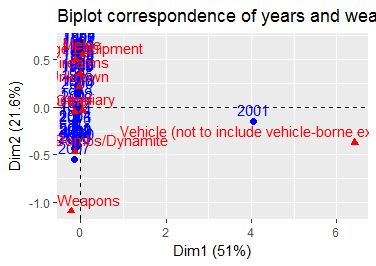
\includegraphics[width=15cm]{Peters_experiment_markdown_files/figure-latex/Rplot_CABIPLOT.png}
\caption{Biplot CA of contingency table of deaths by weapons and year.}
\label{fig:biplotweaponsyears}
\centering
\end{figure}

\begin{figure}[t]
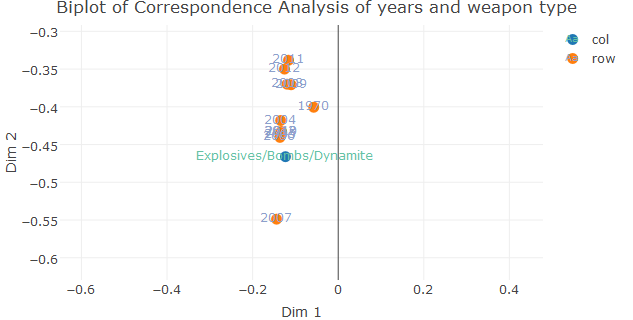
\includegraphics[width=15cm]{Peters_experiment_markdown_files/figure-latex/biplot_zoomin.png}
\caption{Biplot CA of contingency table of deaths by weapons and year, created using Plotly, zoomed in.}
\label{fig:biplotweaponsyearsplotlyzoomin}
\centering
\end{figure}

\begin{figure}[t]
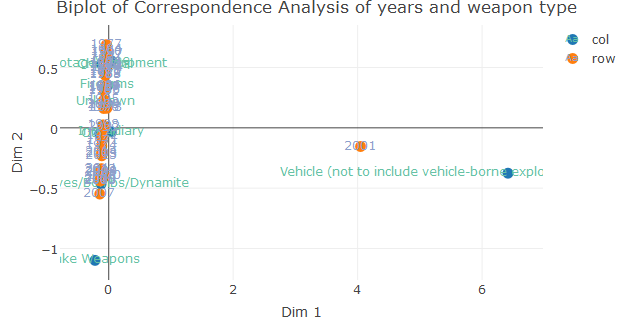
\includegraphics[width=15cm]{Peters_experiment_markdown_files/figure-latex/biplot_zoomout.png}
\caption{Biplot CA of contingency table of deaths by weapons and year, created using Plotly, zoomed in.}
\label{fig:biplotweaponsyearsplotlyzoomout}
\centering
\end{figure}

\subsection{Correspondence analysis of attack type by year}\label{viewing-deaths-by-attack-vector-type-CA}

CA was used understand better both the relationship year and attack type. The contingency table of number of deaths by years and weapon type is shown in table \ref{tab:attacksyear}. From the Biplot , it can be seen that bombings and explosions are strongly associated with 2005 and 2006. Hostage taking or barricade incidents are strongly associated with 1974 and 1998 infrastructure attacks are strongly associated with 2002 and assassinations.


% latex table generated in R 3.3.2 by xtable 1.8-2 package
% Sun Jan 08 11:13:47 2017


\begin{sidewaystable}
\centering
\resizebox{\textwidth}{!}{%
\begin{tabular}{rrrrrrrrrr}
  \hline
 & Armed Assault & Assassination & Bombing/Explosion & Facility/Infrastructure Attack & Hijacking & Hostage Taking (Barricade Incident) & Hostage Taking (Kidnapping) & Unarmed Assault & Unknown \\ 
  \hline
1970 & 36.00 & 15.00 & 96.00 & 9.00 & 1.00 & 0.00 & 10.00 & 0.00 & 4.00 \\ 
  1971 & 14.00 & 73.00 & 79.00 & 1.00 & 0.00 & 0.00 & 2.00 & 0.00 & 4.00 \\ 
  1972 & 58.00 & 208.00 & 281.00 & 1.00 & 5.00 & 0.00 & 12.00 & 0.00 & 1.00 \\ 
  1973 & 41.00 & 171.00 & 75.00 & 0.00 & 34.00 & 38.00 & 11.00 & 0.00 & 0.00 \\ 
  1974 & 34.00 & 161.00 & 289.00 & 0.00 & 1.00 & 35.00 & 14.00 & 1.00 & 7.00 \\ 
  1975 & 225.00 & 211.00 & 136.00 & 0.00 & 0.00 & 35.00 & 8.00 & 0.00 & 2.00 \\ 
  1976 & 160.00 & 231.00 & 222.00 & 6.00 & 27.00 & 16.00 & 8.00 & 0.00 & 2.00 \\ 
  1977 & 141.00 & 140.00 & 33.00 & 2.00 & 107.00 & 1.00 & 22.00 & 0.00 & 10.00 \\ 
  1978 & 318.00 & 255.00 & 317.00 & 434.00 & 0.00 & 52.00 & 25.00 & 7.00 & 51.00 \\ 
  1979 & 599.00 & 505.00 & 582.00 & 44.00 & 0.00 & 20.00 & 81.00 & 3.00 & 266.00 \\ 
  1980 & 2524.00 & 714.00 & 829.00 & 66.00 & 0.00 & 9.00 & 110.00 & 5.00 & 171.00 \\ 
  1981 & 2946.00 & 465.00 & 1045.00 & 39.00 & 9.00 & 8.00 & 51.00 & 1.00 & 287.00 \\ 
  1982 & 3374.00 & 601.00 & 862.00 & 24.00 & 2.00 & 26.00 & 31.00 & 2.00 & 213.00 \\ 
  1983 & 6902.00 & 482.00 & 1624.00 & 19.00 & 0.00 & 1.00 & 29.00 & 0.00 & 386.00 \\ 
  1984 & 6599.00 & 598.00 & 1725.00 & 85.00 & 28.00 & 204.00 & 50.00 & 0.00 & 1160.00 \\ 
  1985 & 4093.00 & 400.00 & 1964.00 & 90.00 & 83.00 & 20.00 & 30.00 & 5.00 & 409.00 \\ 
  1986 & 1920.00 & 461.00 & 1144.00 & 312.00 & 99.00 & 2.00 & 146.00 & 3.00 & 916.00 \\ 
  1987 & 3442.00 & 704.00 & 1730.00 & 9.00 & 1.00 & 6.00 & 68.00 & 21.00 & 497.00 \\ 
  1988 & 4012.00 & 1255.00 & 1710.00 & 28.00 & 12.00 & 1.00 & 79.00 & 1.00 & 94.00 \\ 
  1989 & 4799.00 & 1400.00 & 1741.00 & 16.00 & 3.00 & 21.00 & 101.00 & 2.00 & 38.00 \\ 
  1990 & 4463.00 & 1178.00 & 1015.00 & 10.00 & 10.00 & 0.00 & 395.00 & 22.00 & 55.00 \\ 
  1991 & 5712.00 & 992.00 & 1510.00 & 39.00 & 5.00 & 11.00 & 116.00 & 5.00 & 39.00 \\ 
  1992 & 6154.00 & 1564.00 & 1649.00 & 116.00 & 3.00 & 6.00 & 46.00 & 5.00 & 202.00 \\ 
  1994 & 4375.00 & 1005.00 & 1256.00 & 32.00 & 18.00 & 60.00 & 116.00 & 80.00 & 749.00 \\ 
  1995 & 2256.00 & 852.00 & 1707.00 & 36.00 & 11.00 & 236.00 & 83.00 & 34.00 & 879.00 \\ 
  1996 & 2425.00 & 785.00 & 1627.00 & 16.00 & 5.00 & 147.00 & 95.00 & 11.00 & 1842.00 \\ 
  1997 & 6039.00 & 696.00 & 1742.00 & 48.00 & 0.00 & 4.00 & 125.00 & 8.00 & 2286.00 \\ 
  1998 & 2023.50 & 40.00 & 1607.50 & 39.00 & 1.00 & 0.00 & 338.00 & 101.00 & 528.00 \\ 
  1999 & 1833.00 & 77.00 & 1110.00 & 30.00 & 7.00 & 0.00 & 81.00 & 68.00 & 182.00 \\ 
  2000 & 2008.00 & 214.00 & 1256.00 & 172.00 & 0.00 & 0.00 & 215.00 & 203.00 & 354.00 \\ 
  2001 & 2723.00 & 145.00 & 1019.00 & 133.00 & 3000.00 & 17.00 & 262.00 & 20.00 & 419.00 \\ 
  2002 & 2393.00 & 110.00 & 1754.00 & 1.00 & 6.00 & 170.00 & 106.00 & 10.00 & 249.00 \\ 
  2003 & 1295.00 & 142.00 & 1638.00 & 2.00 & 0.00 & 6.00 & 57.00 & 13.00 & 118.00 \\ 
  2004 & 2103.00 & 170.00 & 3086.00 & 28.00 & 46.00 & 26.00 & 59.00 & 0.00 & 195.00 \\ 
  2005 & 1697.00 & 346.00 & 3922.00 & 16.00 & 12.00 & 0.00 & 141.00 & 4.00 & 173.00 \\ 
  2006 & 2752.00 & 243.00 & 5887.00 & 67.00 & 2.00 & 5.00 & 249.00 & 2.00 & 156.00 \\ 
  2007 & 3183.00 & 190.00 & 8717.00 & 117.00 & 1.00 & 10.00 & 450.00 & 7.00 & 161.00 \\ 
  2008 & 2878.00 & 365.00 & 5211.00 & 37.00 & 19.00 & 0.00 & 336.00 & 16.00 & 231.00 \\ 
  2009 & 2263.00 & 415.00 & 5064.00 & 448.00 & 2.00 & 0.00 & 364.00 & 9.00 & 706.00 \\ 
  2010 & 2014.00 & 484.00 & 4361.00 & 34.00 & 1.00 & 141.00 & 272.00 & 7.00 & 406.00 \\ 
  2011 & 2466.00 & 481.00 & 4575.00 & 46.00 & 2.00 & 7.00 & 276.00 & 6.00 & 339.00 \\ 
  2012 & 5171.29 & 555.33 & 8177.30 & 64.00 & 0.00 & 65.00 & 647.75 & 8.00 & 743.33 \\ 
  2013 & 7331.00 & 829.00 & 12258.83 & 139.00 & 12.00 & 262.00 & 849.50 & 2.00 & 542.67 \\ 
  2014 & 15790.68 & 992.00 & 15529.47 & 351.01 & 27.00 & 276.00 & 7113.00 & 24.00 & 3446.84 \\ 
  2015 & 11702.00 & 1216.00 & 17113.00 & 99.00 & 56.00 & 586.00 & 3175.00 & 32.00 & 4443.00 \\ 
   \hline
\end{tabular}}
\caption{Two way contingency table of Deaths by year and Attack type.}
\label{tab:attacksyear}
\end{sidewaystable}

\begin{figure}[t]
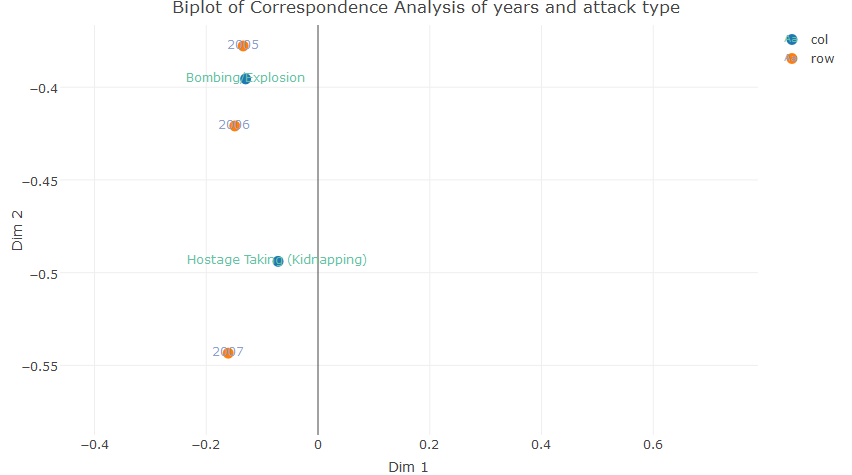
\includegraphics[width=15cm]{Peters_experiment_markdown_files/figure-latex/biplotexlosions.png}
\caption{Biplot CA of contingency table of deaths by attack type and year, created using Plotly, zoomed in to show associations between explosions  and years they occurred.}
\label{fig:biplotattacktypeca1}
\centering
\end{figure}
\begin{figure}[t]
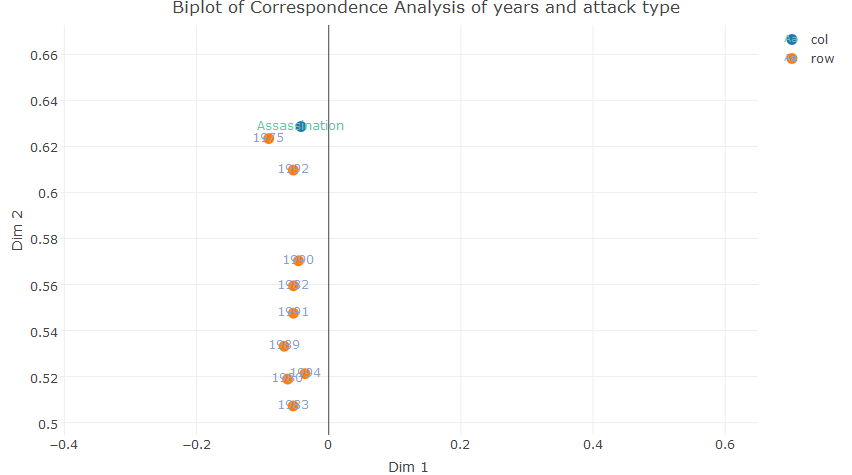
\includegraphics[width=15cm]{Peters_experiment_markdown_files/figure-latex/assassinationbiplot.png}
\caption{Biplot CA of contingency table of deaths by attack type and year, created using Plotly, zoomed in to show associations between assassinations and years they occurred.}
\label{fig:biplotattacktypeca2}
\centering
\end{figure}
\begin{figure}[t]
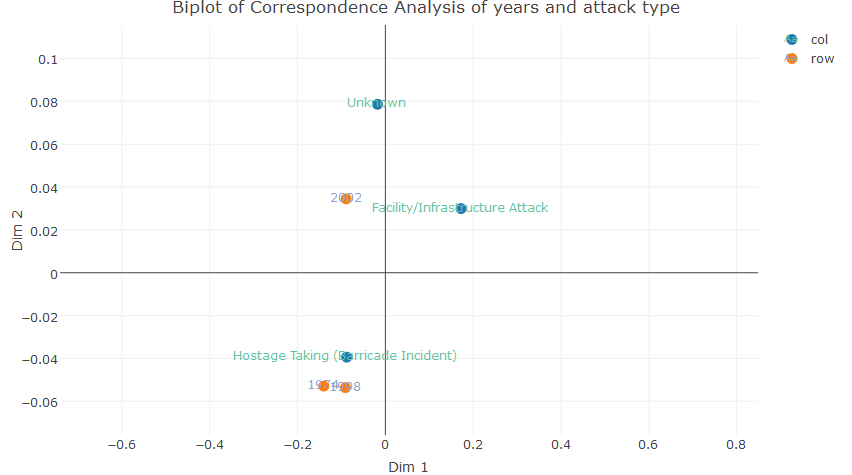
\includegraphics[width=15cm]{Peters_experiment_markdown_files/figure-latex/hostagetakingbiplot.png}
\caption{Biplot CA of contingency table of deaths by attack type and year, created using Plotly, zoomed in to show associations between hostage taking and years they occurred.}
\label{fig:biplotattacktypeca3}
\centering
\end{figure}


\subsection{Multiple Correspondence analysis of terrorist incidents the GTD by year}\label{viewing-deaths-by-attack-vector-type-MCA}

Multiple correspondence analysis (MCA) is an expanded form of correspondence analysis which accommodates the analysis of the relationships between a number of categorical variables. MCA is also known by a number of synonyms including  optimal scaling  or appropriate scoring. Methodologically MCA is carried out by carrying out a atypical CA of an indicator matrix (this is a matrix were the values of individual cells take on values or either 0 or 1). Upon carrying out the CA, the percentages of the explained variance are revised and the inter-point distances which result from the CA are adapted to account for this. Multiple correspondence is an extension of correspondence analysis that allows analysis of multiple variables. Instead of analysis counts of deaths, analysis of terrorist incidents is carried out, the data is also filtered to include only incidents from 'North Africa and the Middle East'. The benefit of using MCA is that the relationship between multiple levels of multiple categorical variables can be examined. A number of incites can be gained from examining the biplot (see figure~\ref{fig:biplotmca}):
\begin{itemize}
\item Examining the biplot one can see the strong association 1974 and terrorist attacks on non state militia or terrorists.
\item Unarmed assaults are strongly associated with chemical weapons use.
\item 2003 are strongly associated with attacks against government, while 2009 shows a strong association between attacks targeting police.  
\item 1994 is strongly associated with attacks using weapon types sabotage equipment and mellee weapons against facilities and infrastructure.
\end{itemize}

\begin{figure}[t]
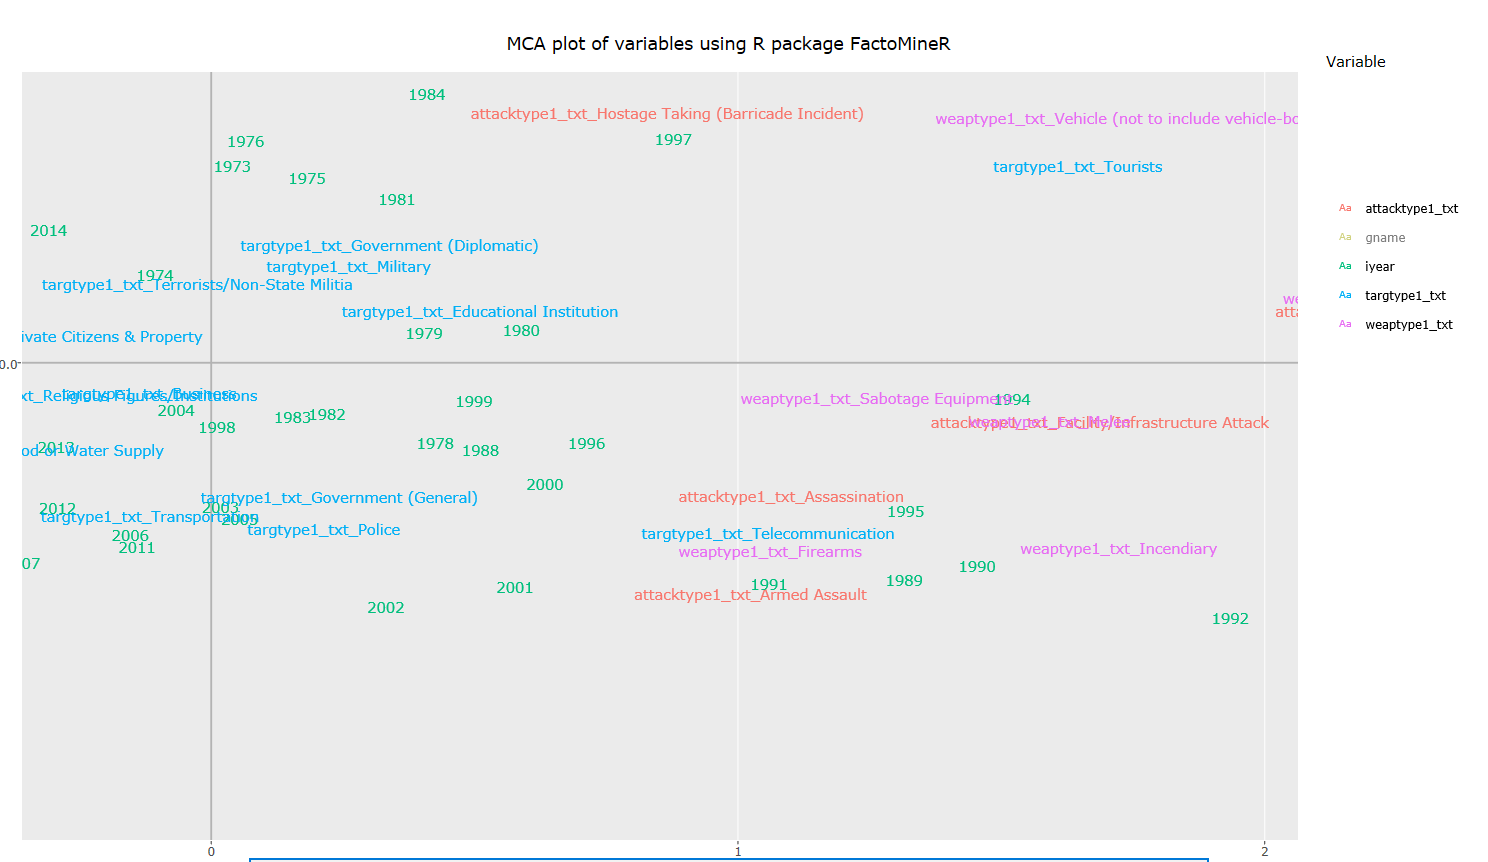
\includegraphics[width=15cm]{Peters_experiment_markdown_files/figure-latex/newplot3.png}
\caption{Biplot of MCA of incidents by attack type, weapon type, target type, group name and year, created using Plotly, zoomed in to show associations between hostage taking and years they occurred.}
\label{fig:biplotmca}
\centering
\end{figure}

\section{Preliminary modelling techniques to gain a temporal understanding of terrorism}
Both Poisson regression and HMM's (Hidden Markov Models) are employed to gain a better understanding of temporal nature of terrorism. While the models utilized are relatively simple they are used aid in the understanding of the temporal nature of terrorism and also to ascertain how events not held in the GTD database can be used to explain the events held within. To do this two separate preliminary studies are carried out, these are:
\begin{itemize}
\item Poisson regression is used model the count of deaths due to terrorism in Iraq in terms of months and major events over the last the period 1970 to 2015. These events are  represented in the timeline chart shown in figure~\ref{fig:timelineiraq}. The aim of carrying out the Poisson regression analysis is to identify what events are affecting the count of deaths due to terrorism. 
\item HMM's are used to model the number of deaths as a time series and the resulting transition state probabilities delivered by the model are used to determine whether the country is in a state of insurgency (transition probability of being in a period of large numbers of daily deaths is high) or in a state of relative calm (transition probability of being in a period of low numbers of daily deaths is high).
\end{itemize}

\section{Poisson, quasi Poisson, Negative Binomial, Linear  and Robust (of log transformed)  regression of deaths due to terrorism in Iraq by month}

Iraq has had a Tumultuous history and in recent years has seen a massive increase in terrorism since the US invasion to overthrow Saddam Hussein's Ba'athist regime, this is visualized in figure~\ref{fig:timelineiraq}. From the timeline plot, one can see a number of key events in Iraq and when the event, both on the timeline but also in terms of the reign of the different governing bodies in Iraq, US and Great Britain. From the time line one can see the following:
\begin{enumerate}
\item The invasion and the US Troop surge took place under Bush regime. The Post surge period and initiation of the draw down of US and NATO troops from Iraq took place.  
\item  Under the Obama administration, the Post surge period continuing into the drawdown of US troops to the eventual pullout of US and NATO troops. The Obama administration was also in place during the rise of ISIS and also the replacement of the Nouri Al Maliki government, which was largely viewed as ineffective (both in terms of effectively managing the country and firstly the fight against Al Qa'ida), \citep{simon2008price} and \citep{kuoti2016exclusion}.
\end{enumerate}

\begin{figure}[t]
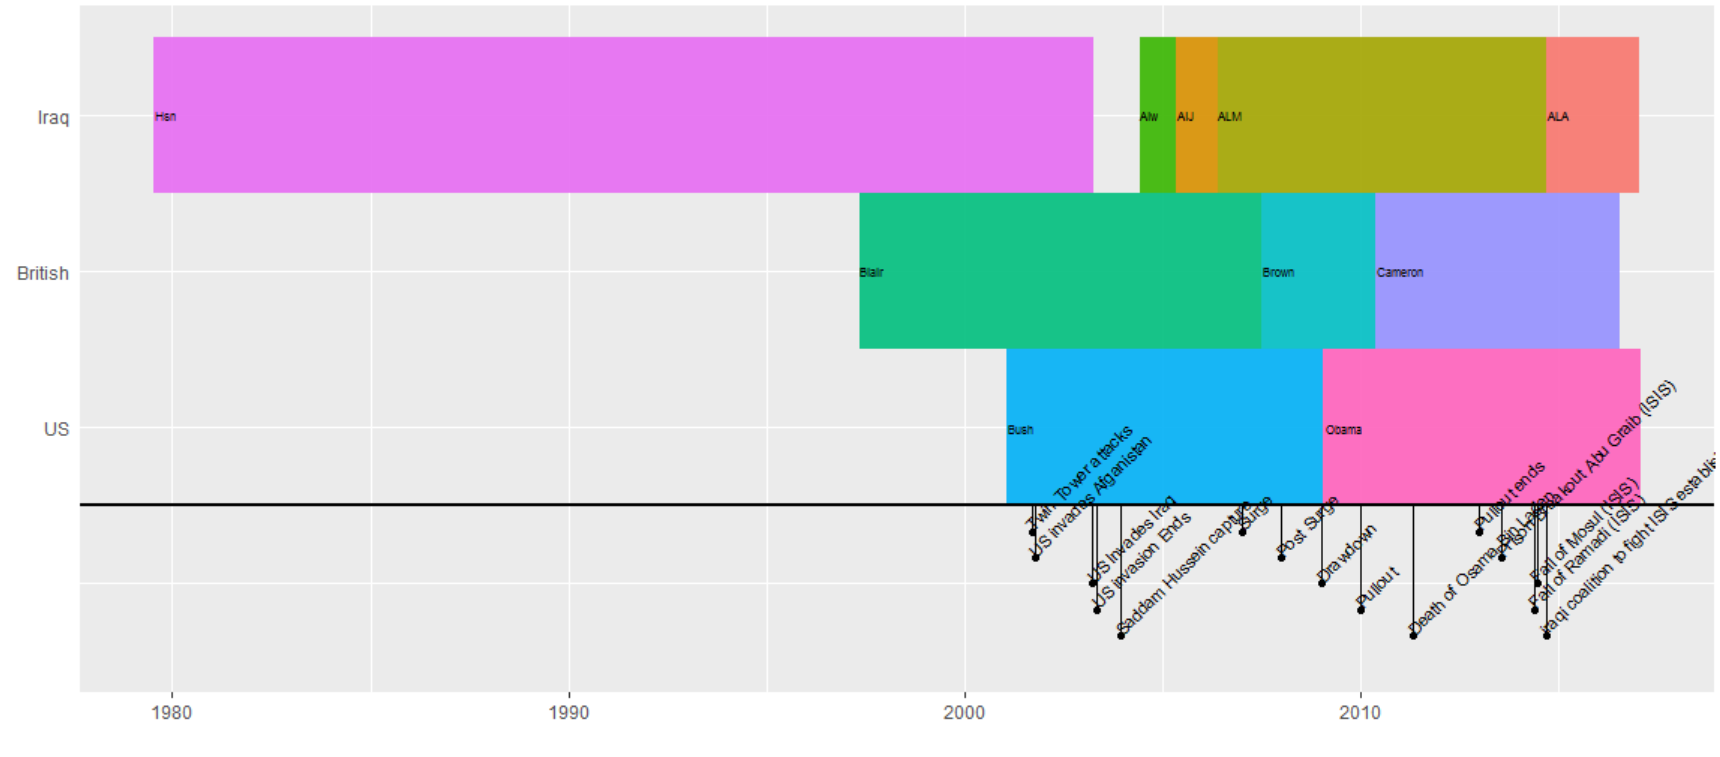
\includegraphics[width=15cm]{Peters_experiment_markdown_files/figure-latex/CaptureTimelineIraq.png}
\caption{Timeline of Iraq post and pre invasion (2003}.
\label{fig:timelineiraq}
\centering
\end{figure}

Over the same period the deaths due to terrorism is shown in figure~ \ref{fig:deathsiniraq}. From the plot of deaths by years for Iraq only it is clear that only after the invasion of Iraq, did the number of deaths due to terrorism. Its also clear from the bar chart that the outbreak of deaths only occurred increased sharply from 2003 to 2007, peaking during the year of the US troop surge.  The preceding years upto 2012 sees a fall off in the number of deaths over this period followed by rise of ISIS \citep{sekulow2015rise} and the resulting civil war in neighbouring Syria. 

\begin{figure}[t]
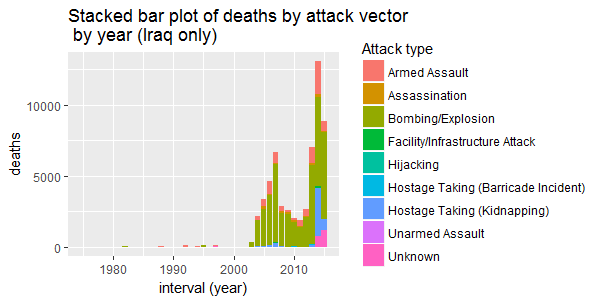
\includegraphics[width=15cm]{Peters_experiment_markdown_files/figure-latex/Rplot01IraqDeaths.png}
\caption{Timeline of Iraq  and US and British presidents and major events since the Iraq invasion.}
\label{fig:deathsiniraq}
\centering
\end{figure}

Poisson regression was first used to model the  monthly death totals due to terrorism in Iraq. Poisson regression is used to model count data, counts are positive integers which represent the number of events which have occurred (in this case it represents the number of deaths due to terrorism). The density distribution for a Poisson distribution is given by the following equation (equation~\ref{eq:poisseqdens}).

\begin{equation} f(y:\mu)= \frac{exp(-\mu)\cdot \mu^y}{y!}  \label{eq:poisseqdens}  \end{equation}

In modelling such events a Poisson distribution is appropriate as the mean is always greater than 0. A random variable has a Poisson distribution if its mean ($mu$)  probability is given by where $mu > 0$. The mean and variance of the distribution can be shown to be equal. As the variance and the mean are equal anything that affects the mean will also affect the variance.In Poisson regression the logarithm of the dependent variable is linked or connected to a linear function of the explanatory variables in such way that (equation~\ref{eq:poisseq}).

\begin{equation} log(y)=Intercept+b_1x_1+b_2x_2...b_nx_n   \label{eq:poisseq}  \end{equation}

Specifically a Poisson regression model, estimates the response variable, the log outcome rate as a linear function of a group of independent variables. Poisson regression makes a number of assumptions about the data. These are:

\begin{itemize}
\item The variable you are trying to predict, the response variable is count data and must be positive.
\item There are one or more predictor variables that are continuous, ordinal or categorical.
\item Independence of observations should be observed in the data, in other words, i.e one observation cannot inform another observation.
\item The distribution of counts being modelled should follow a Poisson distribution. This can be observed by checking the dispersion (for over and under dispersion) of the model. Over dispersion is  were a large amount of variability is observed in the response variable than is predicted using the statistical model. Under dispersion is where there is less variability in the response variable than than in the predicted response.
\end{itemize}

The data was modelled using US and Iraqi president term data, US interventions, terrorism interventions. The summary of table  shows that the model may suffer from a number of a problems. the first parameter of note is the residual deviance of the model. This can be used to calculate a goodness of fit test by carrying out a goodness-of-fit chi-squared test. The null hypothesis of the test is that the model has been specified in a correct manner, however when the test is run the probability  a low probability is obtained  approximately 0, therefore rejecting our null hypothesis that the model is correctly specified. On discovering the Poisson model (and the related quasi-Poisson and Negative binomial) were incorrectly specified, a linear model (as well as a robust linear regerssion model) on log transformed count data was trialled instead. Also a dispersion test is ran and the test clearly shows that the model is strongly over-dispersed.

As stated in the assumptions of Poisson GLMS, for a Poisson GLM the variance and mean are equal, the disperion test \citep{AerRPack} examines whether this assumption (the data is equidispersed) is true or not against the alternative hypothesis  that the variance is equal to the mean \ref{eq:disptest1}.

\begin{equation} VAR[y] = \mu + \alpha * trafo(\mu)   \label{eq:disptest1}  \end{equation}


Where alpha is greater than 0 the model is said to be over-dispersed. As the  model suffered from over dispersion  quasi-poisson regression was used, this methodology does not restrict the dispersion parameter $phi$ to be 1, but is instead  calculated from the data. This has the effect that the coefficient estimates that are calculated from the Poisson model being the same  but the inference from the model is  changed to take account for over dispersion. Examining the summary of the quasi-Poisson, we can see that the residual deviance has not changed. The dispersion parameter which was forced to be 1 when fitting a Poisson regression model is now estimated to be 77.30, indicating over-dispersion. The summary information for both models are shown in tables~\ref{tab:poiss} and \ref{tab:quassipoiss}. 

% Table created by stargazer v.5.2 by Marek Hlavac, Harvard University. E-mail: hlavac at fas.harvard.edu
% Date and time: Tue, Jan 17, 2017 - 20:27:25

\begin{table}[ht] \centering 
  \label{tab:poiss} 
\begin{adjustbox}{width=1\textwidth}
\small  
\begin{tabular}{@{\extracolsep{2pt}}lc} 
\hline \\[-0.8ex] 
 & \multicolumn{1}{c}{\textit{Dependent variable:}} \\ 
\cline{2-2} 
\\[-1.8ex] & kills\_sum \\ 
\hline \\[-1.8ex] 
 month\_since\_1970 & $-$0.0001 \\ 
  & (0.0004) \\ 
 PeriodInherrentresolve & $-$0.556$^{***}$ \\ 
  & (0.081) \\ 
 PeriodPost\_Invasion & 2.122$^{***}$ \\ 
  & (0.249) \\ 
 PeriodPostPullout & $-$0.582$^{***}$ \\ 
  & (0.080) \\ 
 PeriodPre\_Invasion & $-$1.641$^{**}$ \\ 
  & (0.751) \\ 
 PeriodPullout & $-$1.011$^{***}$ \\ 
  & (0.072) \\ 
 PeriodSurge & 2.394$^{***}$ \\ 
  & (0.250) \\ 
 Period\_2ISI driven out of Iraq & $-$0.773$^{***}$ \\ 
  & (0.077) \\ 
 Period\_2ISI founded in Iraq & $-$2.231$^{***}$ \\ 
  & (0.260) \\ 
 Period\_2ISIS breaking wall cmpgn Start & 0.279$^{***}$ \\ 
  & (0.032) \\ 
 Period\_2ISIS cmpgn Soldier Harvest starts & 1.368$^{***}$ \\ 
  & (0.039) \\ 
 Period\_2Maliki sectarian Policies garnishes support for ISIS & $-$0.373$^{***}$ \\ 
  & (0.049) \\ 
 Period\_2None & $-$0.826$^{***}$ \\ 
  & (0.077) \\ 
 Iraq\_PresAyad Allawi & 0.193 \\ 
  & (0.772) \\ 
 Iraq\_PresHaider al-Abadi & 1.976$^{**}$ \\ 
  & (0.812) \\ 
 Iraq\_PresIbrahim Al Jaafari & 0.552 \\ 
  & (0.773) \\ 
 Iraq\_PresIraqi Transition Council & $-$0.734 \\ 
  & (0.771) \\ 
 Iraq\_PresNot stated & $-$1.785$^{**}$ \\ 
  & (0.794) \\ 
 Iraq\_PresNouri al-Malaki & 2.267$^{***}$ \\ 
  & (0.811) \\ 
 Iraq\_PresSaddam Hussein & 0.553$^{*}$ \\ 
  & (0.291) \\ 
 Constant & 3.936$^{***}$ \\ 
  & (0.804) \\ 
Observations & 276 \\ 
Log Likelihood & $-$8,805.310 \\ 
Akaike Inf. Crit. & 17,652.620 \\ 
\hline 
\textit{Note:}  & \multicolumn{1}{r}{$^{*}$p$<$0.1; $^{**}$p$<$0.05; $^{***}$p$<$0.01} \\ 
\end{tabular}
\end{adjustbox} 
\caption{Poisson Regression estimates} 
\end{table}

% Table created by stargazer v.5.2 by Marek Hlavac, Harvard University. E-mail: hlavac at fas.harvard.edu
% Date and time: Tue, Jan 17, 2017 - 20:44:14

\begin{table}[ht] \centering 
  \label{tab:quassipoiss} 
\begin{adjustbox}{width=1\textwidth}
\small 
\begin{tabular}{@{\extracolsep{5pt}}lc} 
\\[-1.8ex]\hline 
\hline \\[-1.8ex] 
 & \multicolumn{1}{c}{\textit{Dependent variable:}} \\ 
\cline{2-2} 
& kills\_sum \\ 
\hline  
 month\_since\_1970 & $-$0.0001 \\ 
  & (0.004) \\
 PeriodInherrentresolve & $-$0.556 \\ 
  & (0.711) \\
 PeriodPost\_Invasion & 2.122 \\ 
  & (2.193) \\
 PeriodPostPullout & $-$0.582 \\ 
  & (0.703) \\
 PeriodPre\_Invasion & $-$1.641 \\ 
  & (6.599) \\
 PeriodPullout & $-$1.011 \\ 
  & (0.636) \\
 PeriodSurge & 2.394 \\ 
  & (2.198) \\
 Period\_2ISI driven out of Iraq & $-$0.773 \\ 
  & (0.679) \\
 Period\_2ISI founded in Iraq & $-$2.231 \\ 
  & (2.283) \\
 Period\_2ISIS breaking wall cmpgn Start & 0.279 \\ 
  & (0.278) \\
 Period\_2ISIS cmpgn Soldier Harvest starts & 1.368$^{***}$ \\ 
  & (0.346) \\
 Period\_2Maliki sectarian Policies garnishes support for ISIS & $-$0.373 \\ 
  & (0.429) \\
 Period\_2None & $-$0.826 \\ 
  & (0.678) \\
 Iraq\_PresAyad Allawi & 0.193 \\ 
  & (6.792) \\
 Iraq\_PresHaider al-Abadi & 1.976 \\ 
  & (7.138) \\
 Iraq\_PresIbrahim Al Jaafari & 0.552 \\ 
  & (6.799) \\ 
 Iraq\_PresIraqi Transition Council & $-$0.734 \\ 
  & (6.777) \\ 
 Iraq\_PresNot stated & $-$1.785 \\ 
  & (6.981) \\ 
 Iraq\_PresNouri al-Malaki & 2.267 \\ 
  & (7.129) \\ 
 Iraq\_PresSaddam Hussein & 0.553 \\ 
  & (2.563) \\ 
 Constant & 3.936 \\ 
  & (7.070) \\ 
Observations & 276 \\ 
\hline 
\textit{Note:}  & \multicolumn{1}{r}{$^{*}$p$<$0.1; $^{**}$p$<$0.05; $^{***}$p$<$0.01} \\ 
\end{tabular} 
\end{adjustbox}
  \caption{quasi-Poisson Regression estimates} 
\end{table} 

Another alternative  tried was the negative binomial model which is another methodology for modelling count data \citep{ver2007quasi}. This methodology presumes a negative binomial distribution which comes about as a gamma mixture of different Poisson distributions. Its probability density can be estimated using the function~\ref{eq:negbin}:

\begin{equation}  f(y:\mu,\theta)=  (\frac{\Gamma(y+\theta)}{\Gamma(\theta)\cdot y!})\cdot \frac{\mu^y\cdot \theta^\theta}{(\mu+\theta)^{y+\theta}}  \label{eq:negbin}  \end{equation}
where:
\begin{itemize}
\item[] $\mu$ =  mean
\item[] $\theta$ = shape parameter
\item[] $\Gamma\cdot$ = is the gamma function
\end{itemize}

The negative binomial model is available in the MASS package \citep{venables2002random}. The negative binomial models makes the assumption that  the conditional means and the conditional variances are the same. This inequality is accounted for by evaluating a dispersion parameter which is held constant when using Poisson regression. In the case of the negative binomial model the theta value is estimated to be 1.035329979.

From the data (table \ref{tab:negbin} and \ref{tab:poiss}) it can be seen that, twice the difference between log likelihoods of the  Poisson model and the negative binomial model is 14643 with a difference in degrees of freedom of 22, df=22-21=1. The large chi-squared value estimated from the difference in log likelihood would tend to suggests the negative binomial model, which estimates the dispersion parameter, is a more appropriate choice than the Poisson model.Also from examining the summary model of the Poisson (table~\ref{tab:poiss}), quasi-Poisson (table~\ref{tab:quassipoiss}) and negative binomial model (table~\ref{tab:negbin}) that the model with the lowest AIC is the negative binomial model (3011.1). However a goodness of fit test for the negative binomial model performed by comparing the residual deviance compared to the maximum deviance of a perfect model where the predicted values match exactly the observed values, gives a statistically significant result, due to the large residual difference . This would indicate that the model does not fit the data particularly well (though it would appear to be a better fit than either the Poisson or quasi-Poisson model). Finally a linear model (and a robust linear model) was fitted using log transformed count outcomes and analysed using OLS regression \citep{UCLAPoiss}.

% Table created by stargazer v.5.2 by Marek Hlavac, Harvard University. E-mail: hlavac at fas.harvard.edu
% Date and time: Tue, Jan 17, 2017 - 22:54:43
\begin{table}[ht] \centering 
  \label{tab:negbin} 
  \begin{adjustbox}{width=1\textwidth}
\small 
\begin{tabular}{@{\extracolsep{5pt}}lc} 
\\[-1.8ex]\hline 
\hline \\[-1.8ex] 
 & \multicolumn{1}{c}{\textit{Dependent variable:}} \\ 
\cline{2-2} 
\\[-1.8ex] & kills\_sum \\ 
\hline \\[-1.8ex] 
 month\_since\_1970 & 0.001 \\ 
  & (0.001) \\ 
 PeriodInherrentresolve & $-$0.571 \\ 
  & (1.271) \\ 
 PeriodPost\_Invasion & 2.160$^{*}$ \\ 
  & (1.299) \\ 
 PeriodPostPullout & $-$0.589 \\ 
  & (1.230) \\ 
 PeriodPre\_Invasion & $-$1.595 \\ 
  & (1.799) \\ 
 PeriodPullout & $-$1.013 \\ 
  & (1.101) \\ 
 PeriodSurge & 2.426$^{*}$ \\ 
  & (1.380) \\ 
 Period\_2ISI driven out of Iraq & $-$0.748 \\ 
  & (1.151) \\ 
 Period\_2ISI founded in Iraq & $-$2.228 \\ 
  & (1.751) \\ 
 Period\_2ISIS breaking wall cmpgn Start & 0.267 \\ 
  & (0.444) \\ 
 Period\_2ISIS cmpgn Soldier Harvest starts & 1.348$^{**}$ \\ 
  & (0.633) \\ 
 Period\_2Maliki sectarian Policies garnishes support for ISIS & $-$0.361 \\ 
  & (0.528) \\ 
 Period\_2None & $-$0.810 \\ 
  & (1.156) \\ 
 Iraq\_PresAyad Allawi & $-$0.055 \\ 
  & (1.494) \\ 
 Iraq\_PresHaider al-Abadi & 1.718 \\ 
  & (1.924) \\ 
 Iraq\_PresIbrahim Al Jaafari & 0.295 \\ 
  & (1.494) \\ 
 Iraq\_PresIraqi Transition Council & $-$0.974 \\ 
  & (1.431) \\ 
 Iraq\_PresNot stated & $-$2.037 \\ 
  & (1.775) \\ 
 Iraq\_PresNouri al-Malaki & 2.015 \\ 
  & (1.933) \\ 
 Iraq\_PresSaddam Hussein & 0.402 \\ 
  & (0.694) \\ 
 Constant & 3.857$^{*}$ \\ 
  & (2.193) \\ 
\hline \\[-1.8ex] 
Observations & 276 \\ 
Log Likelihood & $-$1,484.564 \\ 
$\theta$ & 1.035$^{***}$  (0.101) \\ 
Akaike Inf. Crit. & 3,011.127 \\ 
\hline 
\hline \\[-1.8ex] 
\textit{Note:}  & \multicolumn{1}{r}{$^{*}$p$<$0.1; $^{**}$p$<$0.05; $^{***}$p$<$0.01} \ 
\end{tabular}
\end{adjustbox}
\caption{Negative binomial regression estimates} 
\end{table} 

Before carrying out the linear regression model the response variable is log transformed. The model is then created and the specification is checked by examining the fit output. The general linear f-test applied to our model tests the assumption that the fit of the intercept only model is decidedly less than that of the fit of the model trained. From the summary table the calculated F-statistic is 72.3 (on 20 and 255 degrees of freedom) and the resulting p value is $< 2.2e-6$, suggesting we reject the null hypothesis and accept the alternative hypothesis that the model fit is significantly better than that of the intercept only model. The $R^2$ value obtained from the model is  0.8501 and the residual standard error which is the positive square root of the mean square error, this is calculated to be 0.9778 on 255 degrees of freedom. The model output is shown in table~\ref{tab:linearreg}.To check if our model is specified correctly, a series of diagnostic plots are created to check for the following criteria :
\begin{itemize}
\item Linearity. The relationship between the predictor variables and the response is linear.
\item Homoescadicity. There should be no relationship between the variation in the predictor variables and the error.
\item Independence. The error values are not a caused by any neighbouring values.
\item The error term is normally distributed.
\end{itemize}

To Check if the assumptions made by the linear model are met a number of diagnostic plots are run. First a plot of the residuals versus the fitted values are plotted. While no clear patterns are visible from the residuals versus fitted plot and while the residual are not evenly spread around the line but instead they are clustered together around the midpoint and either extremes of the horizontal line. However a u-shape indicative of a non linear relationship is not observed. 

% Table created by stargazer v.5.2 by Marek Hlavac, Harvard University. E-mail: hlavac at fas.harvard.edu
% Date and time: Wed, Jan 18, 2017 - 23:39:11
\begin{table}[ht] \centering 
\begin{adjustbox}{width=1\textwidth}
\small 
\begin{tabular}{@{\extracolsep{5pt}}lc} 
\\[-1.8ex]\hline 
\hline \\[-1.8ex] 
 & \multicolumn{1}{c}{\textit{Dependent variable:}} \\ 
\cline{2-2} 
\\[-1.8ex] & log(kills\_sum + 1) \\ 
\hline \\[-1.8ex] 
 month\_since\_197503 & 0.004$^{***}$ \\ 
  & (0.001) \\
 PeriodInherrentresolve & $-$1.772 \\ 
  & (1.262) \\
 PeriodPost\_Invasion & 2.293$^{*}$ \\ 
  & (1.268) \\
 PeriodPostPullout & $-$1.800 \\ 
  & (1.221) \\
 PeriodPre\_Invasion & $-$0.587 \\ 
  & (1.627) \\
 PeriodPullout & $-$2.017$^{*}$ \\ 
  & (1.093) \\
 PeriodSurge & 2.539$^{*}$ \\ 
  & (1.350) \\
 Period\_2ISI driven out of Iraq & $-$1.811 \\ 
  & (1.142) \\
 Period\_2ISI founded in Iraq & $-$3.152$^{*}$ \\ 
  & (1.723) \\
 Period\_2ISIS breaking wall cmpgn Start & 0.342 \\ 
  & (0.440) \\
 Period\_2ISIS cmpgn Soldier Harvest starts & 1.513$^{**}$ \\ 
  & (0.629) \\
 Period\_2Maliki sectarian Policies garnishes support for ISIS & $-$1.133$^{**}$ \\ 
  & (0.523) \\
 Period\_2None & $-$1.663 \\ 
  & (1.148) \\
 Iraq\_PresAyad Allawi & 0.130 \\ 
  & (1.269) \\
 Iraq\_PresHaider al-Abadi & 1.873 \\ 
  & (1.733) \\
 Iraq\_PresIbrahim Al Jaafari & 0.340 \\ 
  & (1.269) \\
 Iraq\_PresIraqi Transition Council & $-$1.142 \\ 
  & (1.197) \\
 Iraq\_PresNot stated & $-$1.779 \\ 
  & (1.577) \\
 Iraq\_PresNouri al-Malaki & 2.128 \\ 
  & (1.744) \\
 Iraq\_PresSaddam Hussein & $-$0.637 \\ 
  & (0.625) \\
 Constant & 3.247 \\ 
  & (2.030) \\
\hline \\[-1.8ex] 
Observations & 276 \\ 
R$^{2}$ & 0.850 \\ 
Adjusted R$^{2}$ & 0.838 \\ 
Residual Std. Error & 0.978 (df = 255) \\ 
F Statistic & 72.304$^{***}$ (df = 20; 255) \\ 
\hline 
\hline \\[-1.8ex] 
\textit{Note:}  & \multicolumn{1}{r}{$^{*}$p$<$0.1; $^{**}$p$<$0.05; $^{***}$p$<$0.01} \\ 
\end{tabular} 
\end{adjustbox}
\caption{Linear regression model estimates.} 
\label{tab:linearreg} 
\end{table} 

Secondly a Q-Q plot is plotted to see if the residuals are normally distributed. A Q-Q plot is a plot used to check for normality. By plotting the theoretical quantiles (for a normal distribution) against the actual one can see how well the residuals approximate the normal distribution. While very few points deviate from the line very much. Thirdly a scale location plot is is created to check for Homoescadicity, i.e. that the residuals are spread out evenly across the different values of the predictors \citep{neter1996applied}. While the spread of residuals do not  spread out as much along the x-axis the horizontal red line is fairly straight and the residuals do appear to be randomly spread out. No Clear pattern is observed in the data and a sloped line either up or down indicating Heteroescadicity is observed. Finally a residual versus leverage plot is run to check if any influential cases which may be present in the data are affecting the fit of our model and as such are extremely influential \citep{sall1990leverage}.  If these pints exist they are located in the upper and lower right hand corners. Cooks distance \citep{chatterjee2009sensitivity} which is used to check for the presence of outliers is denoted in Figure~.

A robust regression analysis \citep{rousseeuw2005robust} was then run to check if the linear model was correctly specified. The model coefficients are shown in table~\ref{tab:robustreg}. Robust regression methods are created to be not overly sensitive by violations of assumptions by the underlying data-generating process. The residual standard error (0.4984) on 255 degrees of freedom and the weighted $R^2$ value of 0.9590327. A robust F-test is computed for each predictor in the robust regression model and the output is shown in table.

% Table created by stargazer v.5.2 by Marek Hlavac, Harvard University. E-mail: hlavac at fas.harvard.edu
% Date and time: Wed, Jan 18, 2017 - 23:35:43
\begin{table}[ht] \centering 
  \label{tab:robustreg} 
\begin{adjustbox}{width=1\textwidth}
\small 
\begin{tabular}{@{\extracolsep{5pt}}lc} 
\\[-1.8ex]\hline 
 & \multicolumn{1}{c}{\textit{Dependent variable:}} \\ 
\cline{2-2} 
\\[-1.8ex] & log(kills\_sum + 1) \\ 

 month\_since\_197503 & 0.004$^{***}$ \\ 
  & (0.001) \\ 
 PeriodInherrentresolve & $-$1.772 \\ 
  & (1.262) \\ 
 PeriodPost\_Invasion & 2.293$^{*}$ \\ 
  & (1.268) \\ 
 PeriodPostPullout & $-$1.800 \\ 
  & (1.221) \\ 
 PeriodPre\_Invasion & $-$0.587 \\ 
  & (1.627) \\ 
 PeriodPullout & $-$2.017$^{*}$ \\ 
  & (1.093) \\
 PeriodSurge & 2.539$^{*}$ \\ 
  & (1.350) \\
 Period\_2ISI driven out of Iraq & $-$1.811 \\ 
  & (1.142) \\
 Period\_2ISI founded in Iraq & $-$3.152$^{*}$ \\ 
  & (1.723) \\
 Period\_2ISIS breaking wall cmpgn Start & 0.342 \\ 
  & (0.440) \\
 Period\_2ISIS cmpgn Soldier Harvest starts & 1.513$^{**}$ \\ 
  & (0.629) \\
 Period\_2Maliki sectarian Policies garnishes support for ISIS & $-$1.133$^{**}$ \\ 
  & (0.523) \\
 Period\_2None & $-$1.663 \\ 
  & (1.148) \\
 Iraq\_PresAyad Allawi & 0.130 \\ 
  & (1.269) \\
 Iraq\_PresHaider al-Abadi & 1.873 \\ 
  & (1.733) \\
 Iraq\_PresIbrahim Al Jaafari & 0.340 \\ 
  & (1.269) \\
 Iraq\_PresIraqi Transition Council & $-$1.142 \\ 
  & (1.197) \\
 Iraq\_PresNot stated & $-$1.779 \\ 
  & (1.577) \\
 Iraq\_PresNouri al-Malaki & 2.128 \\ 
  & (1.744) \\
 Iraq\_PresSaddam Hussein & $-$0.637 \\ 
  & (0.625) \\
 Constant & 3.247 \\ 
  & (2.030) \\
\hline \\[-1.8ex] 
Observations & 276 \\ 
R$^{2}$ & 0.850 \\ 
Adjusted R$^{2}$ & 0.838 \\ 
Residual Std. Error & 0.978 (df = 255) \\ 
F Statistic & 72.304$^{***}$ (df = 20; 255) \\ 
\hline 
\hline \\[-1.8ex] 
\textit{Note:}  & \multicolumn{1}{r}{$^{*}$p$<$0.1; $^{**}$p$<$0.05; $^{***}$p$<$0.01} \\ 
\end{tabular}
\end{adjustbox}
\caption{Robust regression estimates.}  
\end{table} 

A robust F-Test is then performed on each of the coefficients of the model to test the importance of the predictor variables. The values are listed in table~\ref{tab:robustregFtest}. From the table we can see that the variables that are significant level (at p $0.05$) are from Period 1 (which refers to periods of major US activity in Iraq) the surge and the post invasion period.  Period 2 which (relates  to periods of major activity by Insurgent groups) is to ISIS soldiers harvest  campaign which was launched in August 2013 by ISIS. From the coefficients in table~\ref{tab:robustregFtest}, we can see that the US troop surge of 2007 is correlated with a major increase in  deaths due to terrorism. This had the opposite effect of what has been seen previously. The effect of different British counter terrorist initiatives has been evaluated by LaFree, \citep{lafree2009impact}. Using the GTD the researchers investigated the effects of different initiatives by the British government throughout the troubles to stop terrorist activity. Six different prominent counter terrorist strategies utilized by the British government from 1969 to 1992 were evaluated using statistical tests to evaluated whether upon applying the intervention did the future risk of attacks rise, reduce or remain the same. similarly major offensives by insurgent groups are correlated with increase in deaths due to terrorism. From the analysis of the regression analysis, both major military interventions by Both sides would appear to be highly correlated with deaths due to terrorism. 

\begin{table}[ht]
  \label{tab:robustregFtest}
\begin{adjustbox}{width=1\textwidth}
\small    
\centering
\begin{tabular}{rlll}
  \hline
 & Variable & F-Statistic & p value \\ 
  
1 & (Intercept) & 2.02359823810467 & 0.156093879216133 \\ 
  2 & month\_since\_197503 & 36.0776198110256 & 6.50364162802437e-09 \\ 
  3 & PeriodInherrentresolve & 0.414977642935234 & 0.52003281066751 \\ 
  4 & PeriodPost\_Invasion & 7.98158258115534 & 0.00509935808610932 \\ 
  5 & PeriodPostPullout & 0.495448791030915 & 0.482148984041935 \\ 
  6 & PeriodPre\_Invasion & 0.423624669339769 & 0.515719967204547 \\ 
  7 & PeriodPullout & 1.82680821883129 & 0.177702751846541 \\ 
  8 & PeriodSurge & 7.82192873483884 & 0.00555489425458082 \\ 
  9 & Period\_2ISI driven out of Iraq & 0.408322169955938 & 0.523395889899178 \\ 
  10 & Period\_2ISI founded in Iraq & 3.33519486191744 & 0.0689816032713713 \\ 
  11 & Period\_2ISIS breaking wall cmpgn Start & 0.515202644885829 & 0.473552347608327 \\ 
  12 & Period\_2ISIS cmpgn Soldier Harvest starts & 7.00367404446488 & 0.00864025159758107 \\ 
  13 & Period\_2Maliki sectarian Policies garnishes support for ISIS & 0.219122961166581 & 0.64010883757994 \\ 
  14 & Period\_2None & 0.796198164498034 & 0.373073733563684 \\ 
  15 & Iraq\_PresAyad Allawi & 0.0264225397673897 & 0.871001402559836 \\ 
  16 & Iraq\_PresHaider al-Abadi & 1.78888890793696 & 0.182253313611277 \\ 
  17 & Iraq\_PresIbrahim Al Jaafari & 0.012027010991077 & 0.912759148623237 \\ 
  18 & Iraq\_PresIraqi Transition Council & 2.493262194502 & 0.115574154436575 \\ 
  19 & Iraq\_PresNot stated & 3.9611969609461 & 0.0476282486970668 \\ 
  20 & Iraq\_PresNouri al-Malaki & 2.34609447269646 & 0.126836955725164 \\ 
  21 & Iraq\_PresSaddam Hussein & 3.01154659984654 & 0.0838814672952424 \\ 
   \hline
\end{tabular}
\end{adjustbox}
\caption{Robust regression robust F-test results.}
\end{table}

\section{Using Hidden Markov Models to analyse the number of daily death due to terrorism}
Hidden Markov Models (HMM's)are a common machine learning approach for modelling time series data. They have seen wide usage and have application in everything from robotics \citep{ladd2005robotics}, speech recognition \citep{gales1998maximum}, genetics for sequence modelling \citep{sonnhammer1998pfam} and financial applications for modelling financial markets \citep{gales1998maximum} and \citep{park2009forecasting}. They can be be viewed as a certain type of dependent mixture model were $X^(t)$ the process subordinate to the state and $C^(t)$ the unobserved parameter process which meets the Markov process. A process is said to to meet the Markov property if conditioning on the previous states in a process up to a time $t$ is the same as conditioning only upto the last value up to of $C_t$ (the transition state probabilities is shown in equation~\ref{eq:markovproca}).

\begin{equation} P_r(C_t+1|C_t,...,C_t)=Pr(C_{t+1}|C_t)  \label{eq:markovproca}  \end{equation}

In a HMM the state dependent process (represented by $X^(t)$) the distribution of $X_t$ is only dependent upon the on the present state of $C_t$ and is not related to earlier or preceding states. These relationships can be summarized as (the transition state probabilities are given by equations \ref{eq:hmm1a},\ref{eq:hmm1b}).

\begin{equation} Pr(C_t|C^{(t-1)})=Pr(C_t|C_{t-1})  \label{eq:hmm1a}  \end{equation}

\begin{equation} Pr(X_t|X^{(t-1)},C^{(t)})=Pr(X_t|C_{t})   \label{eq:hmm1b}  \end{equation}


However the state at time t of the  hidden state is dependent upon previous states. The probability mass function of $X_t$ of the Markov chain being in state i at time t is then given by the formula~\ref{eq:hmm2} 

\begin{equation} p_{i}(x)=Pr(X_{t}=x|C_{t}=t)  \label{eq:hmm2}  \end{equation}

Where $p_i$ represents the probability of $Xt$ of the Markov chain (extracted from the HMM) in state i at time t.

In the exploratory analysis HMM's were built utilizing the depmix S4 package \citep{visser2012package}. Depmix S4  is an R package and infrastructure which allows for the specification and building of HMM's along with the decoding of the models. Depmix S4 carries out  optimization either using using Expectation maximization or alternately through Rdonlp2, which is an R interface to the DONLP2 (Do nonlinear Programming) \citep{spelluccidonlp} software which is used to solve non linear programming problems. When using depmixS4 a model is firstly specified using the depmixS4 function. The Depmix S4 package also allows for a number of distributions to be utilised for the state depending process, those incorporated into the package include binomial, gamma and normal distributions. Depmix S4 offers the user a number of advantages to the analyst including allowing them to utilize inclusion of covariates in state and state dependent process and also the ability to produce synthesized data from the model.

The daily death counts due to terrorism was modelled and a 2 state HMM was trained on the data to predict to different insurgency epochs or regimes (one of relative calm and small numbers of deaths due to terrorism and the second an epoch were there is a high number of deaths due to terrorism). The forward backward algorithm is then used to determine the probability of being in a particular state at any particular moment in time \citep{austin1991forward}. The forward backward algorithm  is an inference algorithm used to determine the posterior marginals of all the hidden state based upon a succession of observations. 

Regime detection is often used in financial time series modelling to aid in deciding a particular strategy to use. These models are used  to detect whether markets are in particular periods such as bull or bear (a bull market is where prices are expected to rise and bear markets are periods or epochs which are characterized by pessimism and falling prices are expected) periods. HMM’s are often used to detect such market periods or regimes, \citep{RegimeDetection2012} and \citep{bae2014dynamic}. The use of HMM's for regime detection would be considered a form of unsupervised learning. Regime detection would be of particular use when deciding which particular anti-terrorist strategy to deploy, does the current situation require deployment of troops or is a draw down of troops required as they are no longer needed to bolster the civilian powers. To this end a HMM was fitted to the terrorism death count data on a dataset derived from GTD pertaining to Iraq. A HMM was specified (using a Gaussian distribution) and fitted on the daily death counts. Two states are specified in the model. The transition state probabilities are then extracted from the model and joined to the death count data and the resulting dataframe is then transformed from wide to long format. Creating a faceted plot of the number of deaths, transition state PS1. 

The transition state probabilities are plotted faceted against the daily death counts due to terrorism (see figure~\ref{fig:Rplot02_hmm_2003_2004}). From figure~\ref{fig:Rplot02_hmm_2003_2004}, it can be seen that state 1 (PS1) that periods with a high probability of being in PS1 are in a regime or epoch of low terrorism. While periods with a high probability of being in state 2 (PS2) refers to a  regime or epoch of high terrorism. Looking at particular time periods the plot become more useful. Examining the plot for 2003 - 2004 (figure~\ref{fig:Rplot02_hmm_2003_2004}), the probability being in a state was very low, up until July of that year when the probability of it being in this state was high, after that time the probability of PS2 was rare but appeared to become more frequent as the year continued. Looking at 2004-2005 (figure~\ref{fig:Rplot02_2004_2005}), as the year went on the frequency of a high probability of PS2 (relating to a terror state) increases. Looking at 2005-2006 (figure~\ref{fig:Rplot02_2005_2006}), as the year went on the frequency of a high probability of PS2 (relating to a terror state)again increases, again this trend continues into 2006-2007 (figure~\ref{fig:Rplot02_2006_2007}). During the period of the US troop surge (2007 to 2008, figure~\ref{fig:Rplot02_2007_2008} and \ref{fig:Rplot02_2008_2009}) again the frequency of PS2 again increases. However  from 2009 to 2011 (figures~\ref{fig:Rplot02_2009_2010}, \ref{fig:Rplot02_2010_2011_HMM} and \ref{fig:Rplot02_2011_2012} ), the frequency of being in PS2 becomes less and less. This begins to change in August 2012, when the frequency of being in PS2 begins to increase again. This trend starts to increase dramatically  in 2013 and by the end of 2013 and 2014 (figures~\ref{fig:Rplot02_2012_2013_HMM} and \ref{fig:Rplot02_2013_2014_HMM})  the frequency of being in PS2 is very frequent.  

Using the state probabilities its possible to discern change points, where you are seeing a major shift from one observed state to another. The methodology shows great potential a a means of identifying outbreaks of terror and possible sudden shifts in (temporal) regime, from a state of 'low terror' to a state of 'high terror.'

\begin{figure}[t]
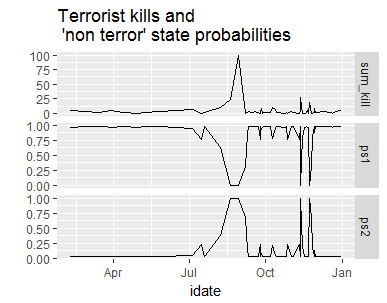
\includegraphics[width=15cm]{Peters_experiment_markdown_files/figure-latex/Rplot02_2003_2004.png}
\caption{Faceted plot of daily death count and probability of emission states due to terrorism from Iraq modelled using a HMM, 2003-2004.}
\label{fig:Rplot02_hmm_2003_2004}
\centering
\end{figure}

\begin{figure}[t]
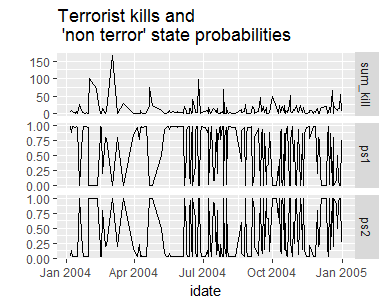
\includegraphics[width=15cm]{Peters_experiment_markdown_files/figure-latex/Rplot02_2004_2005.png}
\caption{faceted plot of daily death count and probability of emission states due to terrorism from Iraq modelled using a HMM, 2004-2005.}
\label{fig:Rplot02_2004_2005}
\centering
\end{figure}

\begin{figure}[t]
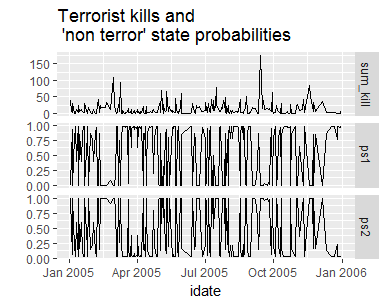
\includegraphics[width=15cm]{Peters_experiment_markdown_files/figure-latex/Rplot02_2005-2006_hmm.png}
\caption{faceted plot of daily death count and probability of emission states due to terrorism from Iraq modelled using a HMM, 2005-2006.}
\label{fig:Rplot02_2005_2006}
\centering
\end{figure}

\begin{figure}[t]
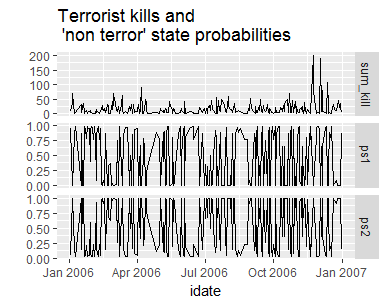
\includegraphics[width=15cm]{Peters_experiment_markdown_files/figure-latex/Rplot02_2006_2007.png}
\caption{faceted plot of daily death count and probability of emission states due to terrorism from Iraq modelled using a HMM, 2006-2007.}
\label{fig:Rplot02_2006_2007}
\centering
\end{figure}

\begin{figure}[t]
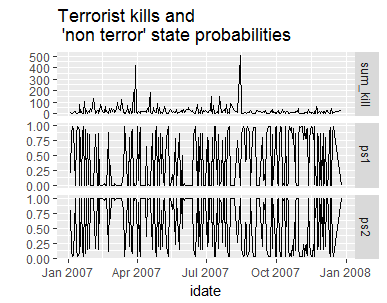
\includegraphics[width=15cm]{Peters_experiment_markdown_files/figure-latex/Rplot02_2007_2008.png}
\caption{faceted plot of daily death count and probability of emission states due to terrorism from Iraq modelled using a HMM, 2007-2008.}
\label{fig:Rplot02_2007_2008}
\centering
\end{figure}

\begin{figure}[t]
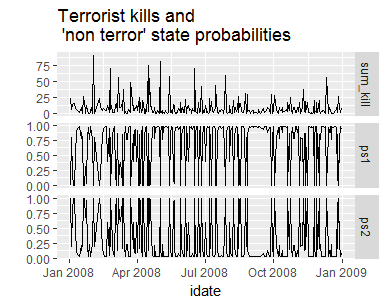
\includegraphics[width=15cm]{Peters_experiment_markdown_files/figure-latex/Rplot02_200_2009.png}
\caption{faceted plot of daily death count and probability of emission states due to terrorism from Iraq modelled using a HMM, 2008-2009.}
\label{fig:Rplot02_2008_2009}
\centering
\end{figure}

\begin{figure}[t]
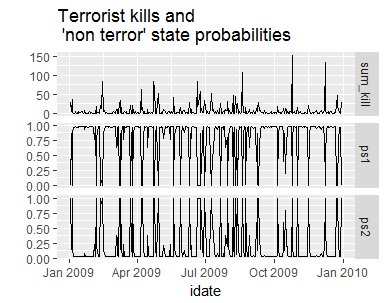
\includegraphics[width=15cm]{Peters_experiment_markdown_files/figure-latex/Rplot02_2009_2010.png}
\caption{faceted plot of daily death count and probability of emission states due to terrorism from Iraq modelled using a HMM, 2009-2010.}
\label{fig:Rplot02_2009_2010}
\centering
\end{figure}

\begin{figure}[t]
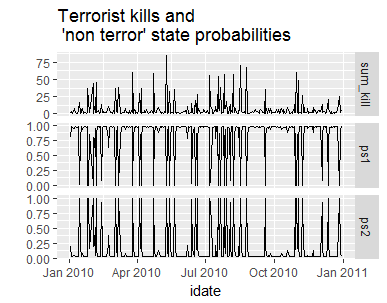
\includegraphics[width=15cm]{Peters_experiment_markdown_files/figure-latex/Rplot02_2010_2011_HMM.png}
\caption{faceted plot of daily death count and probability of emission states due to terrorism from Iraq modelled using a HMM, 2010-2011.}
\label{fig:Rplot02_2010_2011_HMM}
\centering
\end{figure}

\begin{figure}[t]
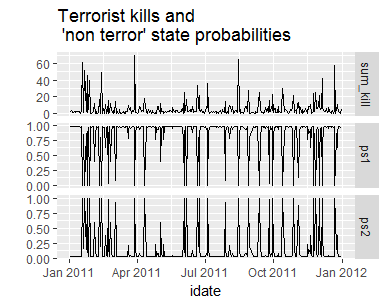
\includegraphics[width=15cm]{Peters_experiment_markdown_files/figure-latex/Rplot02_2011_2012.png}
\caption{faceted plot of daily death count and probability of emission states due to terrorism from Iraq modelled using a HMM, 2011-2012.}
\label{fig:Rplot02_2011_2012}
\centering
\end{figure}

\begin{figure}[t]
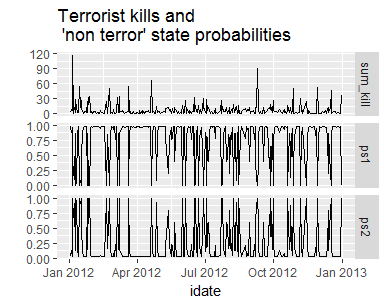
\includegraphics[width=15cm]{Peters_experiment_markdown_files/figure-latex/Rplot02_2012_2013_HMM.png}
\caption{faceted plot of daily death count and probability of emission states due to terrorism from Iraq modelled using a HMM, 2012-2013.}
\label{fig:Rplot02_2012_2013_HMM}
\centering
\end{figure}

\begin{figure}[t]
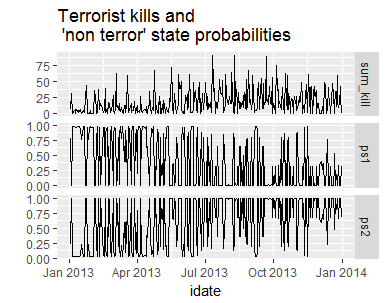
\includegraphics[width=15cm]{Peters_experiment_markdown_files/figure-latex/Rplot02_2013_2014.png}
\caption{faceted plot of daily death count and probability of emission states due to terrorism from Iraq modelled using a HMM, 2013-2014.}
\label{fig:Rplot02_2013_2014_HMM}
\centering
\end{figure}

\section{Overview}

The aim of the section as a preliminary examination of the data was two fold:
\begin{itemize}
\item Firstly to gain a understanding of underlying trends in the data and the relationships between the data.
\item Secondly to ascertain which modelling techniques may be appropriate to the data and which would need further consideration.
\end{itemize}
A mix of descriptive data visualizations, regio and regio temporal visualizations, dimension reduction and the resulting visualization of the dimensions. Preliminary modelling of count  of deaths due to terrorism (country specific to Iraq) was carried out.
Time series plots of Descriptive visualizations of temporal relationships between different weapon, attack vector and regions were carried out using stacked bar charts, this allowed visual encodings  of 3 data dimensions. From the resulting data visualization it was clear to see the resulting regio-temporal relationships  and  attack and weapon type. A clear regio-specific trend can be seen, where Western Europe was the predominant region, Central America and South America in the 1980's, Africa in the 1990's and the 2000's dominated by South Asia and the Middle East. 

This view was enhanced by creating a faceted regio-temporal sums of deaths due to terrorism by decade and the individual countries which are the foremost countries are easy to distinguish. There is also a clear temporal relationship between weapon type vector(the foremost attack vectors now being armed assault and bombings and explosions) and attack type (bombings and explosions). 

This understanding was enhanced using dimension reduction techniques (CA and MCA) and interaction between multiple categorical variables can be ascertained. Specifically certain associations can be seen that are not discernible from the descriptive data visualizations. The dimension reduction techniques when used with interactive visualization techniques based upon the D3 framework made this possible as it allowed analysis to be focussed very deeply onto the data and uncover underlying associations between the different levels of the categorical data being examined. The interactive visualization packages plotly, the googlevis and the leaflet (used for geo-visualizations) package proved adept at this.

Cluster analysis was also carried out on terrorist incidents in Iraq and Syria was done on terrorist incidents in Iraq and the incidents (using both kernel density estimation and k-means clustering) appeared to be largely clustered in urban areas. Iraq and Syria were chosen as the descriptive visualization had shown these region of Middle East an North Africa and South Asia and predominately Iraq, Syria and Afghanistan to be predominant in terms of terrorist activity. While cluster analysis (and kernel density estimation) was able to identify (by overlaying the the clusters of the incidents on an interactive map) a rural-urban divide in terms of where incidents occur. However as an unsupervised method, the number of clusters must be empirically derived so its country wide application to look for a global trend of rural urban divide in terms of where terrorist incidents occur would be difficult to do as the optimal k value would have to be ascertained per country.

After carrying out descriptive statisical visualizations, cluster analysis and dimension reduction techniques a number of preliminary modelling techniques were applied to countries in specific regions based on their pre-eminence in terms of terrorism activity (both death count and incident count). These techniques and the choice of preliminary  modelling technique used and their use case was informed by the literature review of current research into terrorism research using electronic event databases concerning terrorism. either using terrorist data to predict or forecast future trends in incidents or else the use of the GTD to help explain the effects of specific strategies. The aim of the preliminary studies  was also to see how universal the application of  a technique would be and what reach it would have, how easy would the techniqe would be to apply to. Another aim of the analysis was to challenge (by confirming or denying) existing conceptions held about terrorism.

Examples of this would be is there a rural-urban divide in terrorist incidents, 
what was the effect of the surge and what,what if any were the underlying reasons for ISIS's rapid rise, was it a inaction by the West or could the GTD even answer this question. What were the limitations of the data or the type of data held in the GTD and how easy it to augment the GTD with other data sources.

Finally some preliminary modelling of count data was done with both regression (and alternative methodologies) analysis and count data on Iraq's counts of deaths due to terrorism to explain the counts of deaths and the interdependencies with particular US, Iraqi or insurgent actions. HMM's were used to carry out a preliminary time series analysis of counts of deaths due to terrorism In Iraq. From analysis of the emitted state probabilities and the frequency of the states it is possible to see particular epoch and a change of epochs from one of relatively low levels of terrorism to another of a high levels of terrorism. The aim of the modelling was two fold to evaluate how effective the modelling tool. Both modelling count data using regression and using using HMM's proved problematic. When modelling count data the count regression models were found found to suffer from issues with them being not specified correctly.  When using Poisson regression (and its related techniques of quasi-Poisson and negative binomial) to model the count data were found to suffer from being either over dispersed or having a poor goodness of fit. Modelling the data using linear regression or robust linear regression also proved problematic.While HMM's proved useful at identifying different epochs (an epoch of high numbers of deaths due to terrorism, or an epoch of low deaths due to terrorism) of terrorist activity and the onset of these epochs. Such a model would have undoubted usefulness from a number of standpoints, such a model would be capable informing risk management and reinsurance decisions (from an insurance underwriting perspective) or from a governmental point of view identifying when to deploy or mobilise armed forces. However these models due to their unsupervised nature would also prove problematic to deploy globally on a country wide basis as much like clustering the number of transition states would have to be empirically derived. However models that would be able to ascertain similar changes in epoch or outbreaks in terrorist activity would be useful in serving as an early warning system or alarm system to analysts in modelling terrorism. 


